%%%%%%%%%%%%%%%%%%%%%%%%%%%%%%%%%%%%%%%%%%%%%%%%%%%%%%%%%%%%%%%%%%%%%%%%%%%%
% AGUJournalTemplate.tex: this template file is for articles formatted with LaTeX
%
% This file includes commands and instructions
% given in the order necessary to produce a final output that will
% satisfy AGU requirements, including customized APA reference formatting.
%
% You may copy this file and give it your
% article name, and enter your text.
%
%
% Step 1: Set the \documentclass
%
%

%% To submit your paper:
\documentclass[draft]{dependencies/agujournal2019}
\usepackage{url} %this package should fix any errors with URLs in refs.
\usepackage{lineno}
\usepackage[inline]{dependencies/trackchanges} %for better track changes. finalnew option will compile document with changes incorporated.
\usepackage{soul}

%% added
\usepackage{multirow}
\usepackage{amsmath}

\linenumbers
%%%%%%%
% As of 2018 we recommend use of the TrackChanges package to mark revisions.
% Add track changes editors
\addeditor{Fernando Aristizabal}

% The trackchanges package adds five new LaTeX commands:
%
%  \note[editor]{The note}
%  \annote[editor]{Text to annotate}{The note}
%  \add[editor]{Text to add}
%  \remove[editor]{Text to remove}
%  \change[editor]{Text to remove}{Text to add}
%
% complete documentation is here: http://trackchanges.sourceforge.net/
%%%%%%%

\drafttrue

%% Enter journal name below.
%% Choose from this list of Journals:
%
% JGR: Atmospheres
% JGR: Biogeosciences
% JGR: Earth Surface
% JGR: Oceans
% JGR: Planets
% JGR: Solid Earth
% JGR: Space Physics
% Global Biogeochemical Cycles
% Geophysical Research Letters
% Paleoceanography and Paleoclimatology
% Radio Science
% Reviews of Geophysics
% Tectonics
% Space Weather
% Water Resources Research
% Geochemistry, Geophysics, Geosystems
% Journal of Advances in Modeling Earth Systems (JAMES)
% Earth's Future
% Earth and Space Science
% Geohealth
%
% ie, \journalname{Water Resources Research}

\journalname{Water Resources Research}


% starts document
\begin{document}


%% Title and Authors
%% ------------------------------------------------------------------------ %%
%  Title
%
% (A title should be specific, informative, and brief. Use
% abbreviations only if they are defined in the abstract. Titles that
% start with general keywords then specific terms are optimized in
% searches)
%
%% ------------------------------------------------------------------------ %%

% Example: \title{This is a test title}
%
%\title{Reducing Horton-Strahler Stream Order Can Enhance Flood Inundation Mapping Skill with Applications for the U.S. National Water Model}
\title{Extending Height Above Nearest Drainage to Model Multiple Fluvial Sources in Flood Inundation Mapping Applications for the U.S. National Water Model}
%
%% ------------------------------------------------------------------------ %%
%
%  AUTHORS AND AFFILIATIONS
%
%% ------------------------------------------------------------------------ %%

% Authors are individuals who have significantly contributed to the
% research and preparation of the article. Group authors are allowed, if
% each author in the group is separately identified in an appendix.)

% List authors by first name or initial followed by last name and
% separated by commas. Use \affil{} to number affiliations, and
% \thanks{} for author notes.
% Additional author notes should be indicated with \thanks{} (for
% example, for current addresses).

% Example: \authors{A. B. Author\affil{1}\thanks{Current address, Antartica}, B. C. Author\affil{2,3}, and D. E.
% Author\affil{3,4}\thanks{Also funded by Monsanto.}}
%
%
\authors{Fernando Aristizabal\affil{1,2,3}, Fernando Salas\affil{3}, Gregory Petrochenkov\affil{1,3}, Trevor Grout\affil{1,3}\thanks{Colorado Basin River Forecast Center, National Weather Service, National Oceanic and Atmospheric Administration, Salt Lake City, UT, USA}, Brian Avant\affil{1,3}, Bradford Bates\affil{1,3}, Ryan Spies\affil{1,3}, Nick Chadwick\affil{3}, Zachary Wills\affil{1,3}, Jasmeet Judge\affil{2}}
%
%
\affiliation{1}{Lynker, Leesburg, VA, USA}
\affiliation{2}{Center for Remote Sensing, Agricultural and Biological Engineering Department, University of Florida, Gainesville, FL, USA}
\affiliation{3}{National Water Center, Office of Water Prediction, National Weather Service, National Oceanic and Atmospheric Administration, Tuscaloosa, AL, USA}
%
%(repeat as many times as is necessary)
%
%% Corresponding Author:
% Corresponding author mailing address and e-mail address:

% (include name and email addresses of the corresponding author.  More
% than one corresponding author is allowed in this LaTeX file and for
% publication; but only one corresponding author is allowed in our
% editorial system.)
%
% Example: \correspondingauthor{First and Last Name}{email@address.edu}
%
\correspondingauthor{Fernando Aristizabal}{fernando.aristizabal@noaa.gov}



%% Keypoints
%% Keypoints, final entry on title page.

%  List up to three key points (at least one is required)
%  Key Points summarize the main points and conclusions of the article
%  Each must be 140 characters or fewer with no special characters or punctuation and must be complete sentences

% Example:
% \begin{keypoints}
% \item	List up to three key points (at least one is required)
% \item	Key Points summarize the main points and conclusions of the article
% \item	Each must be 140 characters or fewer with no special characters or punctuation and must be complete sentences
% \end{keypoints}

\begin{keypoints}
\item The National Water Model produces forecasts at more than 2.8 million river reaches in the United States.
\item OWP FIM produces flood inundation maps by converting discharges to stages and stages to extents and depths.
\item FIM 3 is a modified version of the Height Above Nearest Drainage technique that provides version improvement with FIM 1 and 2.
\end{keypoints}



%% Abstract
% ------------------------------------------------------------------------ %%
%
%  ABSTRACT and PLAIN LANGUAGE SUMMARY
%
% A good Abstract will begin with a short description of the problem
% being addressed, briefly describe the new data or analyses, then
% briefly states the main conclusion(s) and how they are supported and
% uncertainties.

% The Plain Language Summary should be written for a broad audience,
% including journalists and the science-interested public, that will not have 
% a background in your field.
%
% A Plain Language Summary is required in GRL, JGR: Planets, JGR: Biogeosciences,
% JGR: Oceans, G-Cubed, Reviews of Geophysics, and JAMES.
% see http://sharingscience.agu.org/creating-plain-language-summary/)
%
%% ------------------------------------------------------------------------ %%

%% \begin{abstract} starts the second page

\begin{abstract}
Height Above Nearest Drainage (HAND), a drainage normalizing terrain index, is a means able of producing high resolution flood inundation maps (FIMs) from the National Water Model (NWM) at large scales and high resolutions using reach-averaged synthetic rating curves. 
We highlight here that HAND is limited to producing inundation only when sourced from its nearest drainage line, thus lacks the ability to source inundation from multiple fluvial sources.
A version of HAND, known as Generalized Mainstems (GMS), is proposed that discretizes a target stream network into segments of unit Horton-Strahler stream order known as level paths (LP).
The FIMs associated with each independent LP are then mosaiced together, effectively turning the stream network into discrete groups of homogeneous unit stream order by removing the influence of neighboring tributaries.
Improvement in mapping skill is observed by significantly reducing false negatives at river junctions when the inundation extents are compared to FIMs from that of benchmarks.
A more marginal reduction in the false alarm rate is also observed due to a shift introduced in the stage-discharge relationship by increasing the size of the catchments.
We observe that the improvement of this method applied at 4-5\% of the entire stream network to 100\% of the network is about the same magnitude improvement as going from no drainage order reduction to 4-5\% of the network.
This novel contribution is framed in a new open-source implementation that utilizes the latest combination of hydro-conditioning techniques to enforce drainage and counter limitations in the input data.
\end{abstract}
%
\section*{Plain Language Summary}
Flooding is one of the most impactful natural disasters on life and property.
The United States National Water Model (NWM) provides flood forecasts for the entire country so that adequate warnings can be raised to the public to enable safe evacuations and protective measures.
In order to convert flow rates from the NWM to flood inundation maps (FIM), a model, known as Height Above Nearest Drainage (HAND), is used that converts elevation data from height above mean sea-level to height above the nearest river bottom.
This model suffers from issues in mapping performance because inundation sourced from rivers is only considered from the nearest river line.
We developed a technique that mitigates these errors by removing consideration for neighboring tributaries in the relative elevation computation process.
This is done by splitting the stream network into continuous river segments known as level paths (LPs).
These LPs have no tributaries, thus are known to be stream lines with a unit stream order indicating no branching.
HAND is computed independently for each LP and the resulting FIMs are mosaiced together to form one seamless map.
We compared these HAND derived FIMs to maps from physically-based models and found improvement in mapping performance.
%



%%% Suggested section heads:
% \section{Introduction}
%
% The main text should start with an introduction. Except for short
% manuscripts (such as comments and replies), the text should be divided
% into sections, each with its own heading.

% Headings should be sentence fragments and do not begin with a
% lowercase letter or number. Examples of good headings are:

% \section{Materials and Methods}
% Here is text on Materials and Methods.
%
% \subsection{A descriptive heading about methods}
% More about Methods.
%
% \section{Data} (Or section title might be a descriptive heading about data)
%
% \section{Results} (Or section title might be a descriptive heading about the
% results)
%
% \section{Conclusions}

% Introduction
\section{Introduction}

Flooding is one of the most significant natural disasters in the United States (US) affecting both the loss of life and property. 
In 2017 and 2019, river and flash flooding combined represented the leading cause of death among all natural disasters and second to deaths from heat wave in 2018 \cite{national_weather_service_2020,national_weather_service_2019,national_weather_service_2018}. 
More than an average of 104 deaths per year are attributed to flood events from the 10 year period ending in 2019 \cite{us_department_of_commerce_2020}. 
Within that 10 year window, the most common activity victims were partaking in was driving when compared to other common activities leading to death \cite{us_department_of_commerce_2020}.
With respect to property damages, river and flash flooding have contributed to 60.7, 1.6, and 3.7 billion non-inflation adjusted US dollars in the annual periods of 2017 to 2019, respectively \cite{national_weather_service_2020,national_weather_service_2019,national_weather_service_2018}. 
The large spike in damages for 2017 can be attributed to the Hurricane Harvey event that primarily affected Texas in August. 
Unencouragingly, the trends related to flood damages and fatalities have been steadily increasing over recent decades. \cite{mallakpour2015changing,downton2005reanalysis,kunkel1999temporal,pielke2000precipitation,corringham2019effect}. 
Some are expecting that the hydrologic cycle will intensify which will lead to more extreme precipitation in some areas along with a greater risk of flooding \cite{tabari2020climate,milly2002increasing,wing2018estimates}. 
Increasing trends in frequency and risk are not uniform across spatial regions with work by \citeA{slater2016recent} indicating that trends are increasing across the US Midwest/Great Lakes region while decreasing in coastal Southeast, Southwest and California.

%%%%%%%%%%%%%%%%%%%%%%%%%%%%%%%%%%%%%%%%%%%%%%%%%%%%%%%%
\subsection{Operational Forecasting}
%%%%%%%%%%%%%%%%%%%%%%%%%%%%%%%%%%%%%%%%%%%%%%%%%%%%%%%%

Operational flood forecasting systems are primary tools in developing accurate forecasts for public awareness prior to life or property damaging events occur. 
One of these operational systems is the Advanced Hydrologic Prediction System (AHPS) maintained by National Oceanic Atmospheric Administration (NOAA) National Weather Service (NWS) with approximately 3,781 forecast points across the US at typically short forecast horizons of 24 or 72 hours \cite{mcenery2005noaa}.
AHPS provides forecasting services in the form of ensemble stream flows at 3,781 forecast points illustrated in Figure \ref{fig:all_ahps_points} and flood inundation maps (FIM) at 188 of those forecast points shown in Figure \ref{fig:fim_ahps_points}.
AHPS implements a series of advances including model calibration techniques \cite{zhang2003hydrologic,hogue2003multi,duan2003global,gupta2003advances,parada2003multi}, distributed modeling approaches \cite{reed2004overall,koren2004hydrology,duan2002results}, ensemble forecasting \cite{day1985extended,seo2000simulation,mullusky2002simplified,herr2002simplified}, enhanced data analysis procedures \cite{mcenery2005noaa}, flood-forecasting inundation maps \cite{cajina2002fldview}, hydraulic routing models \cite{fread1973technique,cajina2002fldview}, and multisensor precipitation techniques \cite{breidenbach1999accounting,kondragunta2001outlier,seo2002real,bonnin1996noaa}.
On an approximate basis, there is only one forecast point every 1,455 km of river and one forecast point with FIM every 29,261 km.
Despite the AHPS advances in operational flood forecasting, it lacks of sufficient spatial coverage and long-range forecast horizons.

\begin{figure}[h!]
\centering
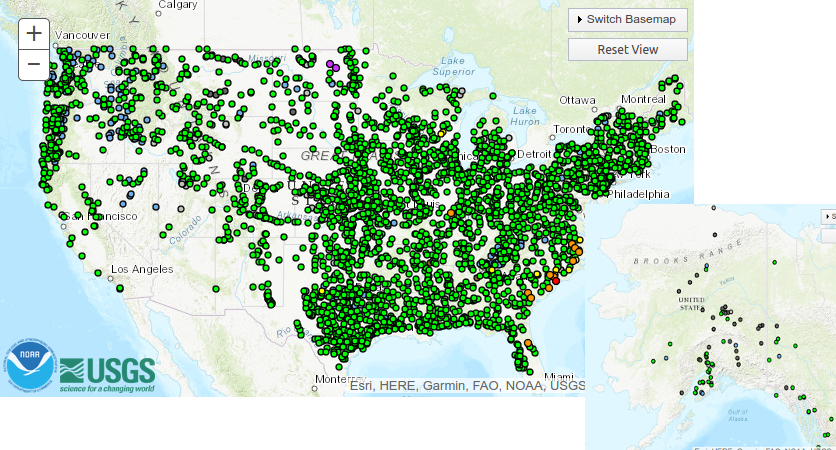
\includegraphics[scale=2.0]{figures/ahps_all_forecast_points.jpg}
\caption{All 3,781 forecast points in United States' Advanced Hydrologic Prediction System for lower 48 states and Alaska. No forecast points in Hawaii or territories. From: water.weather.gov/ahps}
\label{fig:all_ahps_points}
\end{figure}

\begin{figure}[h!]
\centering
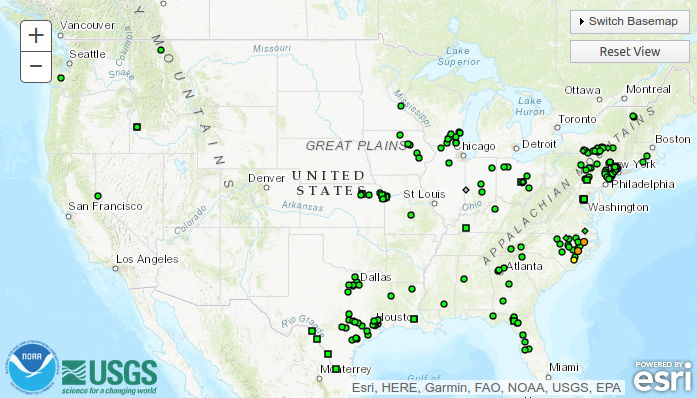
\includegraphics[scale=2.0]{figures/ahps_fim_forecast_points_conus.jpg}
\caption{All 188 forecast points in United States' Advanced Hydrologic Prediction System with flood inundation mapping capabilities. One forecast point near Juneau, Alaska not shown. No forecast points in Hawaii or remaining territories. From: water.weather.gov/ahps}
\label{fig:fim_ahps_points}
\end{figure}

%%%%%%%%%%%%%%%%%%%%%%%%%%%%%%%%%%%%%%%%%%%%%%%%%%%%%%%%
\subsection{National Water Model}
%%%%%%%%%%%%%%%%%%%%%%%%%%%%%%%%%%%%%%%%%%%%%%%%%%%%%%%%

Additional work is required to fill-in the gaps that the AHPS leaves in terms of spatial and temporal coverage.
To broaden the forecasting domain, the Office of Water Prediction (OWP) at the National Water Center (NWC) in Tuscaloosa, Alabama commissioned the development of the National Water Model (NWM) which is an instance of the Weather Research and Forecast Hydrologic Model (WRF-Hydro) \cite{gochis2018wrf,cosgrove2019evolution}. 
The NWM forecasts river discharges at more than 2.7 million forecast points at a variety of time horizons including some medium (10 day) and long (30 day) range forecast horizons.
The NWM enhances but does not replace the spatial and temporal domain of the current AHPS capabilities at the 13 River Forecast Centers (RFC) in areas known as `hydro-blind'. 
It's simply an additional model to be used in the forecasting and early warning decision making.
Furthermore, the NWM as of V1.2 has implemented not only assimilation of real-time United States Geological Survey (USGS) stage discharges but also assimilation of flow forecasts from the AHPS forecast points which are in turn routed downstream and updated whenever a new point is reached. 
This configuration of the NWM is known as `Replace and Route' or `RnR' and is used to enhance the forecasting skill of the NWM with the best available regional-scale data.


The National Hydrography Dataset Plus (NHDPlus) V2.1 is the basis for the hydrofabric in the NWM due to its comprehensive use with the hydrologic communities' stakeholders \cite{mckay2012nhdplus}. 
The term hydrofabric is used within the NWM jargon to describe the subset of hydrography comprised of geospatial datasets required for hydrologic modeling including but not limited to stream networks, catchments, channel properties, and elevation data. 
The Muskingam-Cunge routing method is used within the NWM to reduce computational requirements of a continental scale model \cite{bedient2008hydrology,ponce1994variable,gochis2018wrf}.
Muskingam-Cunge routing scheme has been demonstrated by \citeA{cunge1969subject} to be equivalent to the convective-diffusive wave method without consideration to wave dampening.
As a result of high computational costs and large spatial domains, the need for high-resolution FIM at 10m or better requires additional post-processing from the principal output of the NWM which is forecast river discharges at the reach scale. The Height Above Nearest Drainage (HAND) terrain model is one such technique that can be used, along with synthetic rating curves (SRC), to convert riverine discharges to stages to inundation extents.

%%%%%%%%%%%%%%%%%%%%%%%%%%%%%%%%%%%%%%%%%%%%%%%%%%%%%%%%
\subsection{Height Above Nearest Drainage}
%%%%%%%%%%%%%%%%%%%%%%%%%%%%%%%%%%%%%%%%%%%%%%%%%%%%%%%%
HAND normalizes topography along the nearest drainage path and its been demonstrated to be a good proxy and indicator of a series of important environmental conditions including soil environments, landscape classes, soil gravitational potentials, geomorphologies, soil moisture, and ground water dynamics \cite{renno2008hand,nobre2011height}. 
\citeA{nobre2016hand} showed evidence for utilizing the drainage normalizing HAND dataset as a proxy for flood potential to make static flood inundation maps from known stages.
The terrain index as even gone on to provide additional utility in the observation of riverine flood inundation mapping from remote sensing especially in areas of high electromagnetic interference such as vegetated and anthropogenic areas \cite{aristizabal2020high,shastry2019using,huang2017comparison,twele2016sentinel}.
\citeA{zheng2018river} developed methodology for determine stage-discharge relationships known as synthetic rating curves (SRC) by sampling reach-averaged parameters from HAND datasets and inputting into the Manning's equation \cite{gauckler1867etudes,manning1890flow}.
This collection of methods, coupling HAND with SRCs, has been experimented and compared to other sources of FIM including engineering scale models, in-situ observation, and remote sensing based observation with solid results in large spatial scale applications \cite{godbout2019error,johnson2019integrated,garousi2019terrain,nobre2016hand,afshari2018comparison,zheng2018geoflood,teng2015rapid,teng2017flood,zhang2018comparative}.


Many of those assessing HAND's efficacy for producing FIM have noted opportunities for improvement. 
\citeA{godbout2019error} found how reach length and slope are important parameters for maximizing mapping skill with the moderate values performing best. 
The colinearity of reach length and slope led \citeA{godbout2019error} to propose that reaches of extreme lengths performed worse because of the extreme slope values, a parameter directly represented in Manning's equation. 
Issues with the reach-average approaches have been documented in \citeA{tuozzolo2019impact} where large within reach variance of the roughness Manning's n coefficient have been observed.
These works motivate splitting junction to junction reaches into smaller and equidistant segments for better averaging behavior and SRC representation. 
Furthermore, \citeA{garousi2019terrain} noted improvements to mapping efficacy by conditioning monotonically decreasing thalweg elevations, adjusting the Manning's n roughness coefficient, and using higher resolution (3m) Digital Elevation Model's (DEM) derived from light detection and ranging (Lidar).
Use of higher resolution DEMs in that study was motivated by previous work with Lidar DEMs and least-cost thalweg derivations \cite{zheng2018geoflood}.
Further work by \citeA{johnson2019integrated} noted the general under-prediction of HAND and suggested tuning the Manning's n parameter to better align SRC's with observations. 
Additionally, the sensitivity to low topographic relief and channel slope have been observed \cite{johnson2019integrated,godbout2019error}. 
Catchment boundary issues are noted where the interconnection of catchments are not properly accounted for \cite{zhang2018comparative,mcgehee2016modified}.
These findings suggesting improvements to HAND require advanced computational algorithms and software to compute a FIM hydrofabric required for producing continental-scale FIM (CFIM).

%%%%%%%%%%%%%%%%%%%%%%%%%%%%%%%%%%%%%%%%%%%%%%%%%%%%%%%%
\subsection{HAND Implementations}
%%%%%%%%%%%%%%%%%%%%%%%%%%%%%%%%%%%%%%%%%%%%%%%%%%%%%%%%

Due to significant advances in high-performance computing (HPC) and large scale high-resolution DEM's such as the National Elevation Dataset (NED) at the 10m scale, HAND has been implemented into software for large-scale, continental computation. 
HAND was initially implemented into operational software by the National Flood Interoperability Experiment (NFIE) to generate FIM hydrofabric (will be used interchangeably with the datasets produced by HAND) rapidly on a high-performance computer (HPC) \cite{maidment2017conceptual,liu2016cybergis}. 
NFIE used open-source dependencies including the Terrain Analysis Using Digital Elevation Models (TauDEM) \cite{tarboton2005terrain} and the Geospatial Data Abstraction Library (GDAL) \cite{warmerdam2008geospatial} to compute HAND for the Continental United States (CONUS) at 331 Hydrologic Unit Code (HUC) 6 processing units in 1.34 CPU years.
By allocating 31 nodes at 20 cores per for a total of 620 available cores to the overall operation, it enabled the production to finish up in 36 hours consuming 3.2TB of peak memory and 5TB of total disk space.
Originally, NFIE utilized the National Hydrography Dataset (NHD) Plus Medium Resolution (MR) to etch or burn flowlines prior to further conditioning but more recent work has advanced this to the more current NHDPlus High Resolution (HR) \cite{liu2020height}. 
The original NFIE dataset was employed by the NWC to produce forecast FIM from the NWM for use within its network of RFC's for additional guidance in hydro-blind regions and tagged as OWP's FIM V1.0.
Further work by \citeA{djokic2019arc}, implemented a series of improvements to HAND including equidistant reaches, updates to use with NHDPlusHR hydrography, and AGREE-DEM reconditioning \cite{hellweger1997agree} into an ESRI Arc-Hydro workflow with use in ArcGIS and tagged as OWP FIM V2.0. 
More notably the software added the ability to derive drainage potentials on a per mainstem basis as originally conceptualized by \citeA{mcgehee2016modified}.
Mainstem is generally used here as defined in \citeA{blodgett2020mainstems} but only available in mainstems downstream of forecast AHPS points within the workflow introduced by \citeA{djokic2019arc}.
Overall, the software package is estimated to run CONUS at the full-resolution in 0.55 CPU years in a desktop setting.
In addition to the domestic work done in the US, some studies have expanded upon HAND to cover global domains at 30m resolutions \cite{yamazaki2019merit,donchyts2016global}.

%%%%%%%%%%%%%%%%%%%%%%%%%%%%%%%%%%%%%%%%%%%%%%%%%%%%%%%%
\subsection{OWP FIM 3.0 `Cahaba'}
%%%%%%%%%%%%%%%%%%%%%%%%%%%%%%%%%%%%%%%%%%%%%%%%%%%%%%%%

A study is proposed to introduce and evaluate the development of OWP FIM V3.0 which utilizes some of the latest mapping techniques along with a few novel developments in a computationally friendly framework. 
FIM 3 was asked to meet a series of requirements to enhance its utility for continental scale FIM from the National Water Model for operational forecasting and to ensure long-term success in future developments. 
The requirements were

\begin{enumerate}
\item use easily accessible, open-source dependencies to promote free-use and open-access community development and research.
\item excellent single-core computational and memory performance with favorable, time and space complexities,
\item ability to parallelize across multiple cores and nodes within HPC or cloud compute environments,
\item preprocessing functionality within package pipeline to acquire and process input artifacts,
\item rapid inundation mapping capabilities to go from FIM hydrofabric datasets to forecast FIMs from NWM,
\item automated testing functionality to ensure modifications enhance forecast skill when compared to external sources,
\item ability to produce depth forecasts,
\item full NWM domain coverage (including Hawaii and Puerto Rico),
\item provide initial mitigation to catchment boundary issues at RnR mainstems,
\item and improved FIM forecasting skill when compared to FIM V1.0 and V2.0.
\end{enumerate} 

To meet these higher specifications for the next generation of authoritative FIM capabilities, the OWP FIM V3.0 `Cahaba' was developed. 
It meets all the specifications listed above including version on version improvement of FIM skill due to the implementation of new developments in HAND techniques. 
The following methods and results describe the work in more detail and demonstrates its efficacy in producing enhanced FIM from the NWM for operational forecast applications. 
Furthermore, it enables the contribution from the broader hydro-community as further advances are made in this developing area of research.



%
% Materials and Methods
\clearpage % this clears figures before references
%%%%%%%%%%%%%%%%%%%%%%%%%%%%%%%%%%%%%%%%%%%%%%%%%%%%%%%%
%%%%%%%%%%%%%%%%%%%%%%%%%%%%%%%%%%%%%%%%%%%%%%%%%%%%%%%%
\section{Materials and Methods}
%%%%%%%%%%%%%%%%%%%%%%%%%%%%%%%%%%%%%%%%%%%%%%%%%%%%%%%%
%%%%%%%%%%%%%%%%%%%%%%%%%%%%%%%%%%%%%%%%%%%%%%%%%%%%%%%%
%
FIM 3 is a fully operational pipeline of software tools to help acquire datasets, cache hydrofabrics, produce FIMs, and evaluate results.
%
%%%%%%%%%%%%%%%%%%%%%%%%%%%%%%%%%%%%%%%%%%%%%%%%%%%%%%%%
\subsection{Software Dependencies and Architecture}
%%%%%%%%%%%%%%%%%%%%%%%%%%%%%%%%%%%%%%%%%%%%%%%%%%%%%%%%
%
OWP FIM exclusively utilizes free and open source software dependencies including Python 3, GDAL, TauDEM, Geographic Resource Analysis Support System (GRASS), GNU Parallel, and MPICH \cite{python382,gdal2020,tarboton2005terrain,grass2020,tange2015gnu,amer2021mpich}.
Within the Python 3 ecosystem, many common packages are employed including but not limited RichDEM, GeoPandas, Rasterio, Rasterstats, and Numba \cite{barnes2018richdem,jordahl2014geopandas,lam2015numba}. 
To simplify setup and enhance portability across host operating systems OWP FIM packages all dependencies up in Docker image (\url{https://docs.docker.com/engine/install/}). 
A user only need to install Docker on their host machine and build the image from the provided recipe. 

The FIM 3 pipeline is discretized into key areas that a user can interact with to reproduce the results of this study. Preprocessing acquires and prepares datasets for production of the FIM 3 hydrofabric. 
Producing the FIM hydrofabric produces the datasets required to make an inundation map including the relative elevation model (REM) or HAND grid, the catchments in vector and raster form, and the hydro-table (contains synthetic rating curves and cross-walk information).
%
%%%%%%%%%%%%%%%%%%%%%%%%%%%%%%%%%%%%%%%%%%%%%%%%%%%%%%%%
\subsection{Datasets}
%%%%%%%%%%%%%%%%%%%%%%%%%%%%%%%%%%%%%%%%%%%%%%%%%%%%%%%%
%
All data sources used within FIM 3 are publicly available from a variety of government sources including the USGS, NWC, Federal Emergency Management Agency (FEMA), and US Army Core of Engineers (USACE) to enhance reproducibility and collaboration among government, academia, and industry.
The National Hydrography Dataset Plus High Resolution (NHDPlusHR) Beta Version is the latest hydrography dataset used for land surface hydrologic modeling in the US \cite{moore2019user}. 
It is used in conjunction with the hydrofabric of the NWM V2.1 to help define flowlines for FIM 3 while the NWM hydrofabric is also used to define reservoirs for exclusion and catchments to cross-walk to for forecasting purposes.
The AHPS forecast points are required to determine the RnR downstream segments in order to define the RnR Mainstems (MS).
For enforcing levee data into the NED DEMs, the USACE National Levee Database (NLD) is used via burning feature elevations \cite{engineers2016national}.
Additionally, FEMA Base Level Engineering (BLE) from Region 6 (parts of Texas, Oklahoma, Arkansas, Louisiana and New Mexico) 1\% (100 year) and 0.2\% (500 year) datasets are used as validation in this study. 
These BLE datasets are provided at the watershed scale (HUC8) utilizing best available simulations and DEMs.
The full input datasets sorted by source are listed below:
%
\begin{enumerate}
\item{USGS - NHDPlusHR Beta}
    \begin{enumerate}
    \item{\textit{BurnLineEvents:} flowlines used by NHDPlusHR for hydro-enforcing DEM}
    \item{\textit{Value-Added Attributes:} database of additional attributes referenced to flowlines that enhance navigation, analysis, and display}
    \item{\textit{DEM:} DEM from National Elevation Dataset (NED) in 10m (or 1/3 arc-second) spatial resolution with vertical units in centimeters \cite{gesch2002national}}
    \end{enumerate}
\item{NOAA OWP - NWM V2.1 Hydrofabric}
    \begin{enumerate}
    \item{\textit{flowlines:} stream network center lines used for NWM routing and forecasting}
    \item{\textit{reach level catchments:} surface drainage area corresponding to each river reach}
    \item{\textit{waterbodies:} includes reservoirs, lakes, and others that are modeled within the NWM}
    \end{enumerate}
\item{USACE - NLD}
    \begin{enumerate}
    \item{\textit{Levee elevations:} Top of levee elevations are gathered with in the NLD provided by USACE for hydro-enforcement}
    \end{enumerate}
\item{Land Sea Border}
\item{FEMA BLE}
    \begin{enumerate}
    \item{\textit{cross-sections:} cross-sections and associated data for associating 1\% and 0.2\% recurrence discharges with NWM reaches}
    \item{\textit{flood inundation maps:} FIMs produced by BLE at the two recurrence intervals for comparison with FIMs from OWP FIM versions}
    \end{enumerate}
\item{NOAA OWP - AHPS Forecast Points}
    \begin{enumerate}
    \item{\textit{AHPS:} Collection AHPS forecast points to associate to RnR Mainstems}
    \end{enumerate}
\end{enumerate}
%
%%%%%%%%%%%%%%%%%%%%%%%%%%%%%%%%%%%%%%%%%%%%%%%%%%%%%%%%
\subsection{Hydro-conditioning}
%%%%%%%%%%%%%%%%%%%%%%%%%%%%%%%%%%%%%%%%%%%%%%%%%%%%%%%%
%
The DEM from the NED is subject to a series of hydro-conditioning procedures to enhance it's suitability for riverine flood inundation mapping. 
These techniques are specific for making OWP FIM and differ from the conditioning methods used by the NHDPlusHR Beta \cite{moore2019user}.
Hydro-conditioning is implemented to obtain many objectives including enforcing the location of hydrologically relevant features such as flowlines, lakes, or drainage divides whether natural or anthropogenic. 
It can also be used to simulate more accurate bathymetry which is not accounted for in the NED 10m DEM \cite{gesch2002national}.

Specifically within the context of FIM 3, the hydro-conditioning operations that take place in sequential order are presented. 
Prior to any hydro-conditioning, all input datasets must be subset from their original spatial domain scales into the processing unit designated at run time which can be either HUC 4, 6 or 8. 
The subsetting is done by spatial query for the cases of the levees, DEM, and NWM hydrofabric while the NHDPlusHR BurnLineEvents are subset via attribute query for the given reachcode's membership in the processing unit.
Hydro-conditioning raster operations take place on buffered boundary definitions to avoid edge contamination and effects \cite{lindsay2013measuring}. 
%
%%%%%%%%%%%%%%%%%%%%%%%%%%%%%%%%%%%%%%%%%%%%%%%%%%%%%%%%
\subsubsection{Stream Network Enforcement} 
\label{ssec:stream_network_enforcment}
%
\note[Fernando Aristizabal]{For Brian Avant}
The location of the stream network are enforced to ensure general agreement with established stream networks.
The NHDPlus HR Beta Burnline Event layer is used to enforce stream locations in the NHDPlusHR workflow so it is also used here for hydro-enforcement \cite{moore2019user}. 
However, to better match the drainage density of the NWM V2.1 stream network which is based on the NHDPlus Medium Resolution, the Burnline Events are pruned utilizing a nearest neighbor search around the NWM flowlines. 
Pruning the NHD network is completed at for every NWM V2.1 headwater point, the nearest NHDPlusHR Burline Event feature is selected and downstream features are also selected.
The resulting pruned NHD stream network is what gets hydro-enforced in subsequent operations.
This procedure is best illustrated in Figure \ref{fig:stream_density_pruning} which shows that the pruned NHD network corresponds to the full density NHD network at NWM V2.1 headwater locations only. 
Additionally, the NHDPlusHR pruned headwaters are later used for seeding a new FIM drainage network that best agrees withe DEM after all hydro-conditioning takes place.
%
\begin{figure}[h!]
\centering
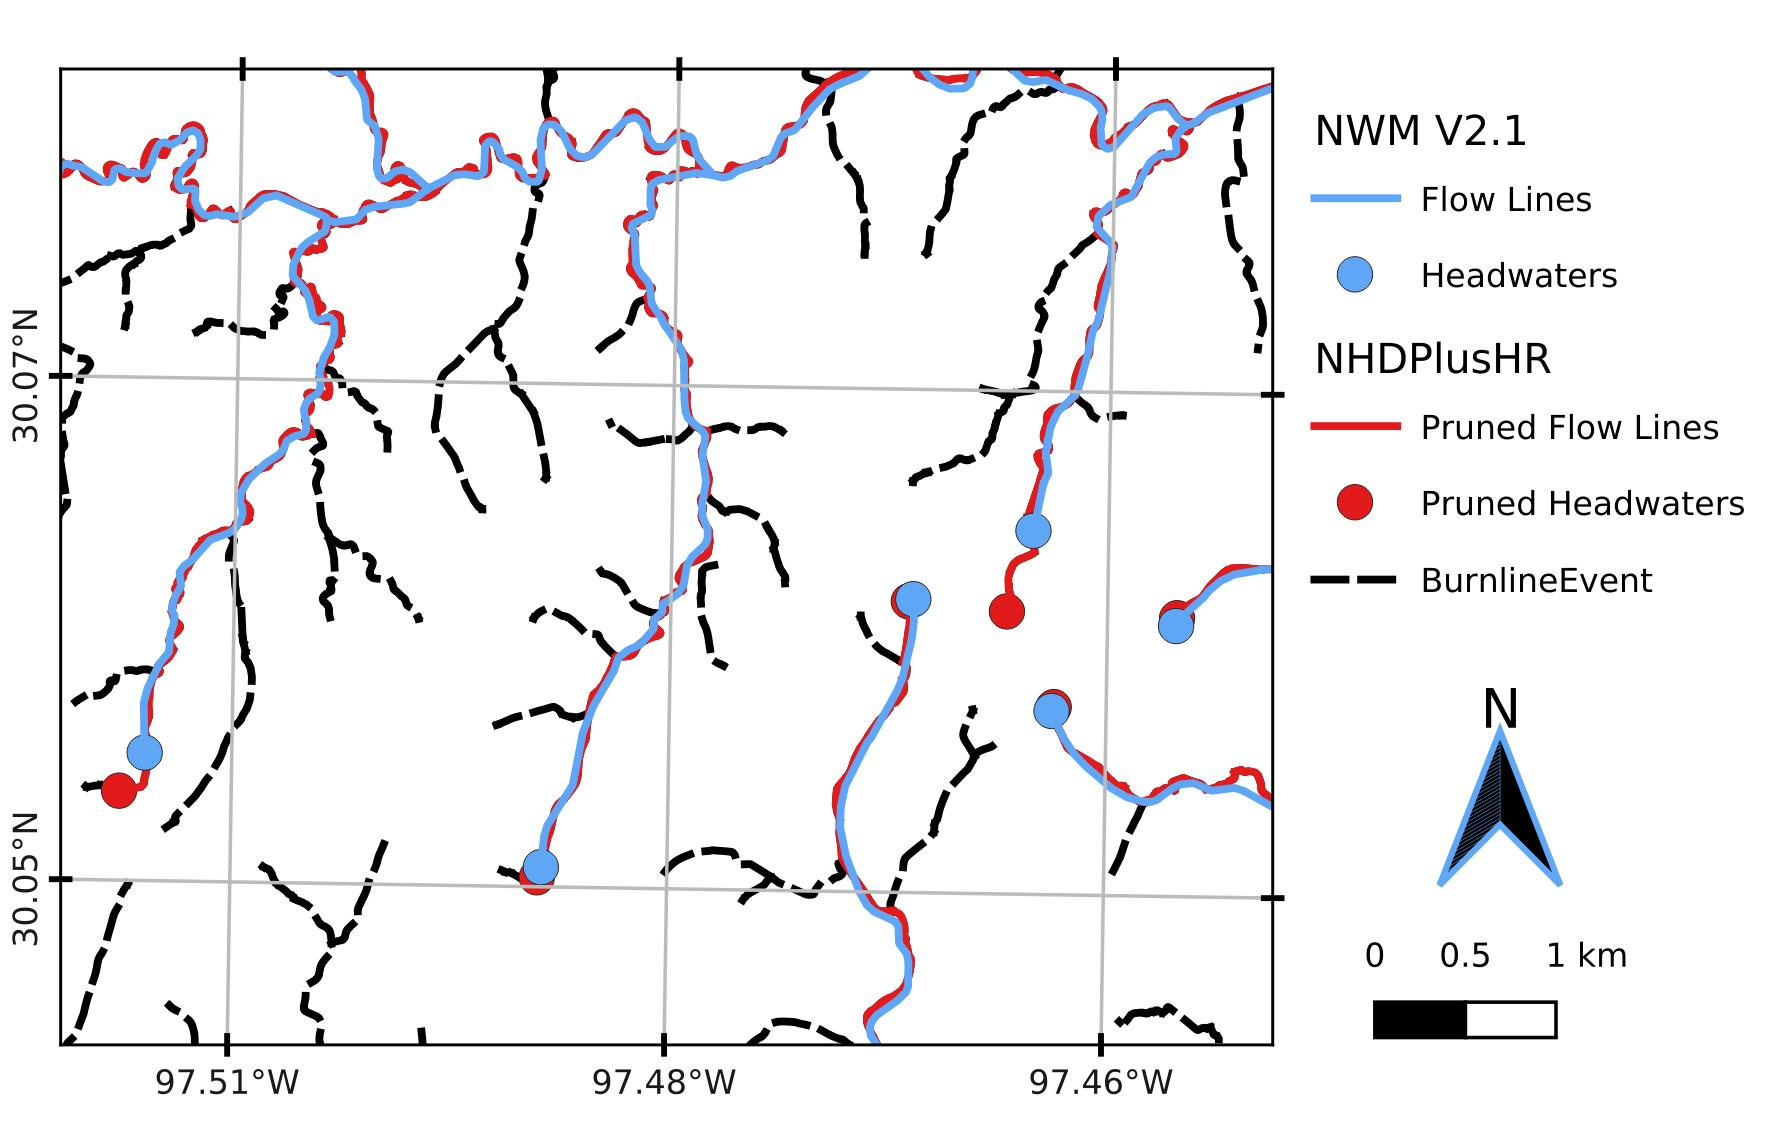
\includegraphics[scale=1.0]{figures/headwaters.jpg}
\caption{Pruning of NHDPlus HR Beta Burnline Events (dotted black) to NWM V2.1 stream density (blue) using nearest neighbor selection. Resulting stream network (red) matches the drainage density of NWM V2.1 while corresponding spatially with the NHDPlusHR Burnline Events.}
\label{fig:stream_density_pruning}
\end{figure}
%
This results in a stream network that has the same density as the NWM V2.1 flowline network but utilizes the locations of the NHDPlusHR Beta BurnLineEvents. 

\note[Fernando Aristizabal]{For Trevor Grout}
The pruned stream network is then utilized to hydro-enforce the DEM with a methodology developed by \citeA{hellweger1997agree} known as the AGREE DEM Surface Reconditioning System. 
The AGREE algorithm seeks to burn artificially deep thalweg elevations by a uniform value known as sharp drop. 
The modification continues by excavating an area of a given buffer distance from the thalweg by a depth proportional to the distance from the channel given by the smooth drop. 
The resulting enforcement of the thalweg and general bathymetric region results in a cross-section resembling a trapezoidal shape with a significantly lower elevation along the thalweg line only as can be seen in Figure \ref{fig:agree_dem_cross_section}.
%
\begin{figure}[h!]
\centering
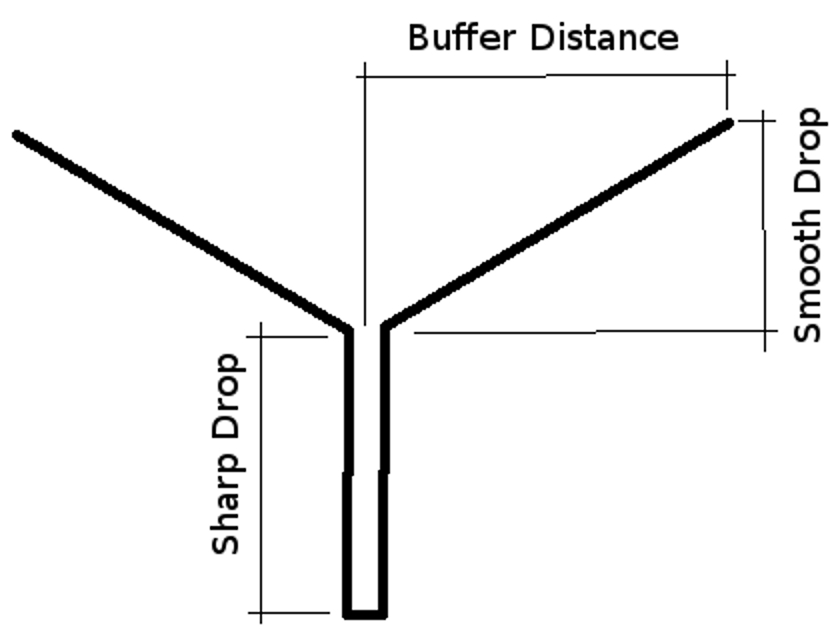
\includegraphics[scale=1.0]{figures/agree_dem_cross_section.jpg}
\caption{Placeholder for AGREE DEM illustration}
\label{fig:agree_dem_cross_section}
\end{figure}
%
In total, the AGREE algorithm requires three parameters including the buffer distance, smooth drop, and sharp drop. 
Using simple thalweg burning techniques as opposed to the full AGREE method helps prevent distortions in the delineation of streams as well as the catchment boundaries \cite{saunders1995grid,saunders1996gis,mizgalewicz1996modeling,hellweger1997agree,quenzer1998gis,baker2006comparison}.
\citeA{baker2006comparison} noted AGREE produced satisfactory results when compared to other enforcement especially when computational costs are considered. 
Downsides to the technique include the possibility of exhibiting parallel streams where the burned stream and real stream are both represented \cite{hellweger1997agree,saunders1999preparation} and some distortion of the catchment boundaries can also be observed \cite{saunders1999preparation,saunders1996gis}. Some of these drawbacks are later addressed by additional conditioning techniques later on.
%
%%%%%%%%%%%%%%%%%%%%%%%%%%%%%%%%%%%%%%%%%%%%%%%%%%%%%%%%
\subsubsection{Levee Enforcement}
%
\note[Fernando Aristizabal]{For Ryan Spies}
The National Elevation Dataset at 10m resolution lacks sufficient representation of fine grain features such as levees and embankments.
In order to better represent the influences of these features upon hydraulics and inundation extents, the National Levee Database (NLD) published by USACE was used to enforce elevations within the 10m DEM.
%
%\begin{figure}[h!]
%\centering
%\includegraphics[scale=1.0]{figures/levee_histogram.jpg}
%\caption{Placeholder for figure demonstrating histogram of elevation differences. May have too many results figures to allow for one}
%\label{fig:levee_histogram}
%\end{figure}
%
%%%%%%%%%%%%%%%%%%%%%%%%%%%%%%%%%%%%%%%%%%%%%%%%%%%%%%%%
\subsubsection{Depression Filling}
%
Local depressions are a naturally occurring features of a DEM but must be addressed if a connected drainage network with continuous catchments are to be derived for flood modeling purposes.
The conditioned DEM was removed of depressions by filling areas with pits while preserving the stream and levee information previously enforced.
Priority-Flood developed by \citeA{barnes2014priority} is an algorithm for filling said depressions and shown to have improved performance over early works in the field by \citeA{jenson1988extracting} implemented in \citeA{tarboton2005terrain} as well as \citeA{planchon2002fast}.
The depression filling algorithm used in our pipeline is a Priority-Flood variant developed by \cite{zhou2016efficient} with enhanced single-thread performance and a time complexity of O(n log n) for floating point grids.
This performance was enabled by limiting the processing queue with a region-growing method to exclude many of the slope cells \cite{zhou2016efficient}.
The depression technique employed here does leave the existence of flat regions where pits existed aprior thus later requiring the need for resolving these flats.
The enhanced variant of Priority-Flood is implemented and made available by \citeA{barnes2018richdem} and \citeA{zhou2015filldem}.
%
%%%%%%%%%%%%%%%%%%%%%%%%%%%%%%%%%%%%%%%%%%%%%%%%%%%%%%%%
\subsubsection{Stream Thalweg Elevation Conditioning}
%
Thalweg elevations are critical components of relative elevation based inundation mapping thus much is performed to ensure the best available, monotonically decreasing elevations are derived prior to normalizing of elevations.
In order to prevent situations where the burned thalweg and the thalweg endemic to DEM run parallel to one another, the normalized excavation algorithm \cite{saunders1999preparation} is used to seek a zonal (nearest neighbor) elevation minimum for each thalweg pixel. 
Each zone is defined as the thalweg's pixel nearest neighborhood within a maximum distance of 50m.
The zonal minimum is computed for each thalweg pixel zone and the minimum is used to replace the existing thalweg elevation value.

The next step involves conditioning these local minimums along the thalweg to enforce monotonically decreasing thalweg elevations for FIM.
\citeA{garousi2019terrain} proposed an algorithm that traverses stream thalweg pixels in a depth first manner starting with adding all the headwater pixels to a queue. 
The connectivity of the thalweg pixels is defined by the D-8 flow directions further discussed in Section \ref{ssec:flow_direction_and_flat_resolution}.
At every thalweg pixel, the minimum elevation among itself and its upstream contributing thalweg pixels is taken as shown in equation \ref{eq:thalweg_breach},
%
\begin{equation}
\label{eq:thalweg_breach}
\textbf{D}[x] = \min_{y\ drains\ to\ x} {(\ \textbf{D}[x]\ ,\ \textbf{D}[y]\ )}
\end{equation}
%
, in which \textbf{D} represents the array of thalweg adjusted elevations indexed by x and y where by y is upstream of x. 
When a pixel's upstream neighbors are all evaluated, the downstream pixel is added into the queue thus the depth first traversal of the drainage network.
This procedure enforces the location of streams and ensures that thalweg elevations are hydrologically correct which yielded a 7\% improvement in critical success index (CSI) per an evaluation for an event in 2017 on the Malad river \cite{garousi2019terrain}.
%
%%%%%%%%%%%%%%%%%%%%%%%%%%%%%%%%%%%%%%%%%%%%%%%%%%%%%%%%
\subsection{Deriving FIM Hydrofabric}
%%%%%%%%%%%%%%%%%%%%%%%%%%%%%%%%%%%%%%%%%%%%%%%%%%%%%%%%
%
%%%%%%%%%%%%%%%%%%%%%%%%%%%%%%%%%%%%%%%%%%%%%%%%%%%%%%%%
\subsubsection{Flow Directions and Flats Resolution}
\label{ssec:flow_direction_and_flat_resolution}
%
To facilitate the generation of a connected stream network and its associated catchments from the conditioned DEM, the depression-filled DEM is used to derive connectivity in the form of D-8 flow directions.
D-8 seeks to allocate a drainage direction for every pixel based on the adjacent eight pixel neighborhood with the steepest slope \cite{o1984extraction}.
The horizontal component of slope is defined as one for the 4 neighboring pixels in the main cardinal directions while the intercardinal pixels are designated a horizontal component of $\sqrt{2}$. 
The flow direction is encoded as integers 1 through 8 corresponding with the cardinal direction East as 1 and continuing counter-clockwise to the Southwest direction as 8. 
Flow directions are derived for non-depression filled regions trivially with the above procedure but to define connectivity for every grid cell the remaining flats corresponding to depression filled cells must be resolved.

Flat resolution from flats endemic to the DEM or from depression filled regions is a costly,non-trivial procedure which was originally addressed by \citeA{garbrecht1997assignment}.  
Software implementations have developed means to partition the problem and resolve flats iteratively with communication across processes \cite{tarboton2009generalized,tesfa2011extraction,wallis2009parallel,tarboton2005terrain}.
The excessive iteration and communication leads to poor computational performance which motivated further work on how to optimize flat resolution \cite{survila2016scalable,barnes2014efficient}.
Specifically the work by \citeA{survila2016scalable} enables the use of parallel processing and made smoother catchments from our informal experience than those from \citeA{barnes2014efficient}.
By processing flats local to each partition separately from flats shared with other partitions, the accelerated flat resolution algorithm demonstrated an average speed up 468x when compared to prior implementations \cite{survila2016scalable}.
OWP FIM 3 utilized a CyberGIS implementation of the D-8 flow direction algorithm with the accelerated resolution of flats \cite{survila2016scalable,cybergis2016}.
%
%%%%%%%%%%%%%%%%%%%%%%%%%%%%%%%%%%%%%%%%%%%%%%%%%%%%%%%%
\subsubsection{Deriving FIM Stream Network}
%
\note[Fernando Aristizabal]{For Brian Avant}
The derivations of relative elevations and catchments from the newly conditioned DEM involves re-deriving a new FIM stream network. 
The FIM stream network is of the same density as the NWM V2.1 network and fully converges at all junctions leaving no divergences in the network.
This is accomplished by using the seed points generated from the stream network enforcement process (Section \ref{ssec:stream_network_enforcment}).
These seeds points are headwater locations of the NHDPlusHR Beta Burnline Events layer that spatially correspond to theheadwater definitions in the stream network of the NWM V2.1.
Feeding the seed points and previously computed flow directions into flow accumulation methods \cite{wallis2009parallel,tarboton1997new,tarboton2005terrain} yields a stream link accumulation raster that can be converted to a vector file for further processing.
Each stream link in this derived FIM stream network is split into equidistant reaches.
Stream links are defined here as segments of rivers discretized by junctions with other NWM river segments.
Stream links are then further segmented at NWM lakes and HUC8 boundaries.
Discretizing at NWM lakes isolates reaches and catchments associated with lakes and reservoirs to avoid mapping them using the Manning's equation and could potentially enable volume based mapping in the future as a feature enhancement.
Additionally every reach (and later catchment) is assigned a globally unique identifier based on the HUC 8 membership.

Now that the stream network has been re-derived using the hydro-conditioning techniques previously discussed, the split stream reaches need to cross-walked to the forecast stream network which is that of the National Water Model's.
%
%%%%%%%%%%%%%%%%%%%%%%%%%%%%%%%%%%%%%%%%%%%%%%%%%%%%%%%%
\subsubsection{Catchments}
%

%
%%%%%%%%%%%%%%%%%%%%%%%%%%%%%%%%%%%%%%%%%%%%%%%%%%%%%%%%
\subsubsection{Relative Elevation Model}
%

%
%%%%%%%%%%%%%%%%%%%%%%%%%%%%%%%%%%%%%%%%%%%%%%%%%%%%%%%%
\subsubsection{Synthetic Rating Curves}
%

%
%%%%%%%%%%%%%%%%%%%%%%%%%%%%%%%%%%%%%%%%%%%%%%%%%%%%%%%%
\subsection{RnR Mainstems Method}
%

%
%%%%%%%%%%%%%%%%%%%%%%%%%%%%%%%%%%%%%%%%%%%%%%%%%%%%%%%%
\subsection{Inundation Mapping}
%

%
%%%%%%%%%%%%%%%%%%%%%%%%%%%%%%%%%%%%%%%%%%%%%%%%%%%%%%%%
\subsection{Evaluation and Testing}
%%%%%%%%%%%%%%%%%%%%%%%%%%%%%%%%%%%%%%%%%%%%%%%%%%%%%%%%
%

%

%
% Results
\clearpage % this clears figures before references
%%%%%%%%%%%%%%%%%%%%%%%%%%%%%%%%%%%%%%%%%%%%%%%%%%%%%%%%
%%%%%%%%%%%%%%%%%%%%%%%%%%%%%%%%%%%%%%%%%%%%%%%%%%%%%%%%
\section{Results}
\label{sec:results}
%%%%%%%%%%%%%%%%%%%%%%%%%%%%%%%%%%%%%%%%%%%%%%%%%%%%%%%%
%%%%%%%%%%%%%%%%%%%%%%%%%%%%%%%%%%%%%%%%%%%%%%%%%%%%%%%%
%
%%%%%%%%%%%%%%%%%%%%%%%%%%%%%%%%%%%%%%%%%%%%%%%%%%%%%%%%
\subsection{Mapping Performance}
\label{ssec:mapping_performance}
%%%%%%%%%%%%%%%%%%%%%%%%%%%%%%%%%%%%%%%%%%%%%%%%%%%%%%%%
%
We produced FIMs for the entire BLE domain within the 49 HUC8 area across several states in the south central US. 
The forecasted FIMs using the discharges for the 1\% (100 year) and 0.2\% (500 year) recurrence flows directly from HEC-RAS were used to avoid noise and errors from hydrological processes.
We computed the statistics (CSI, POD, and FAR) for both 100 and 500 year events for Mannings N set to 0.06 and 0.12. 
The distribution of these statistics can be examined in Figure \ref{fig:violin_plot} as violin plots.
Each half of a violin plot represents the kernel density estimation (KDE) for a given model (FR, MS, GMS), given Manning's n value (0.06, 0.12), and given recurrence interval (1\%, 0.2\%), and performance metric (CSI, POD, FAR).
We also denote trend lines for each metric and Manning's n setting as well as their respective slope estimate and one-tailed p-value denoting the level of significance of the trend.

Aggregating the metrics in the method above treats each HUC8 as it's own unit and does little to consider the size differences of the HUCs. 
In an opposing aggregation method, we illustrate in Table \ref{tab:aggregate_metrics} the sum of all the TPs, FPs, and FNs to recompute CSI, POD, and FAR across the entire domain. 
%
\begin{figure}[h!]
\centering
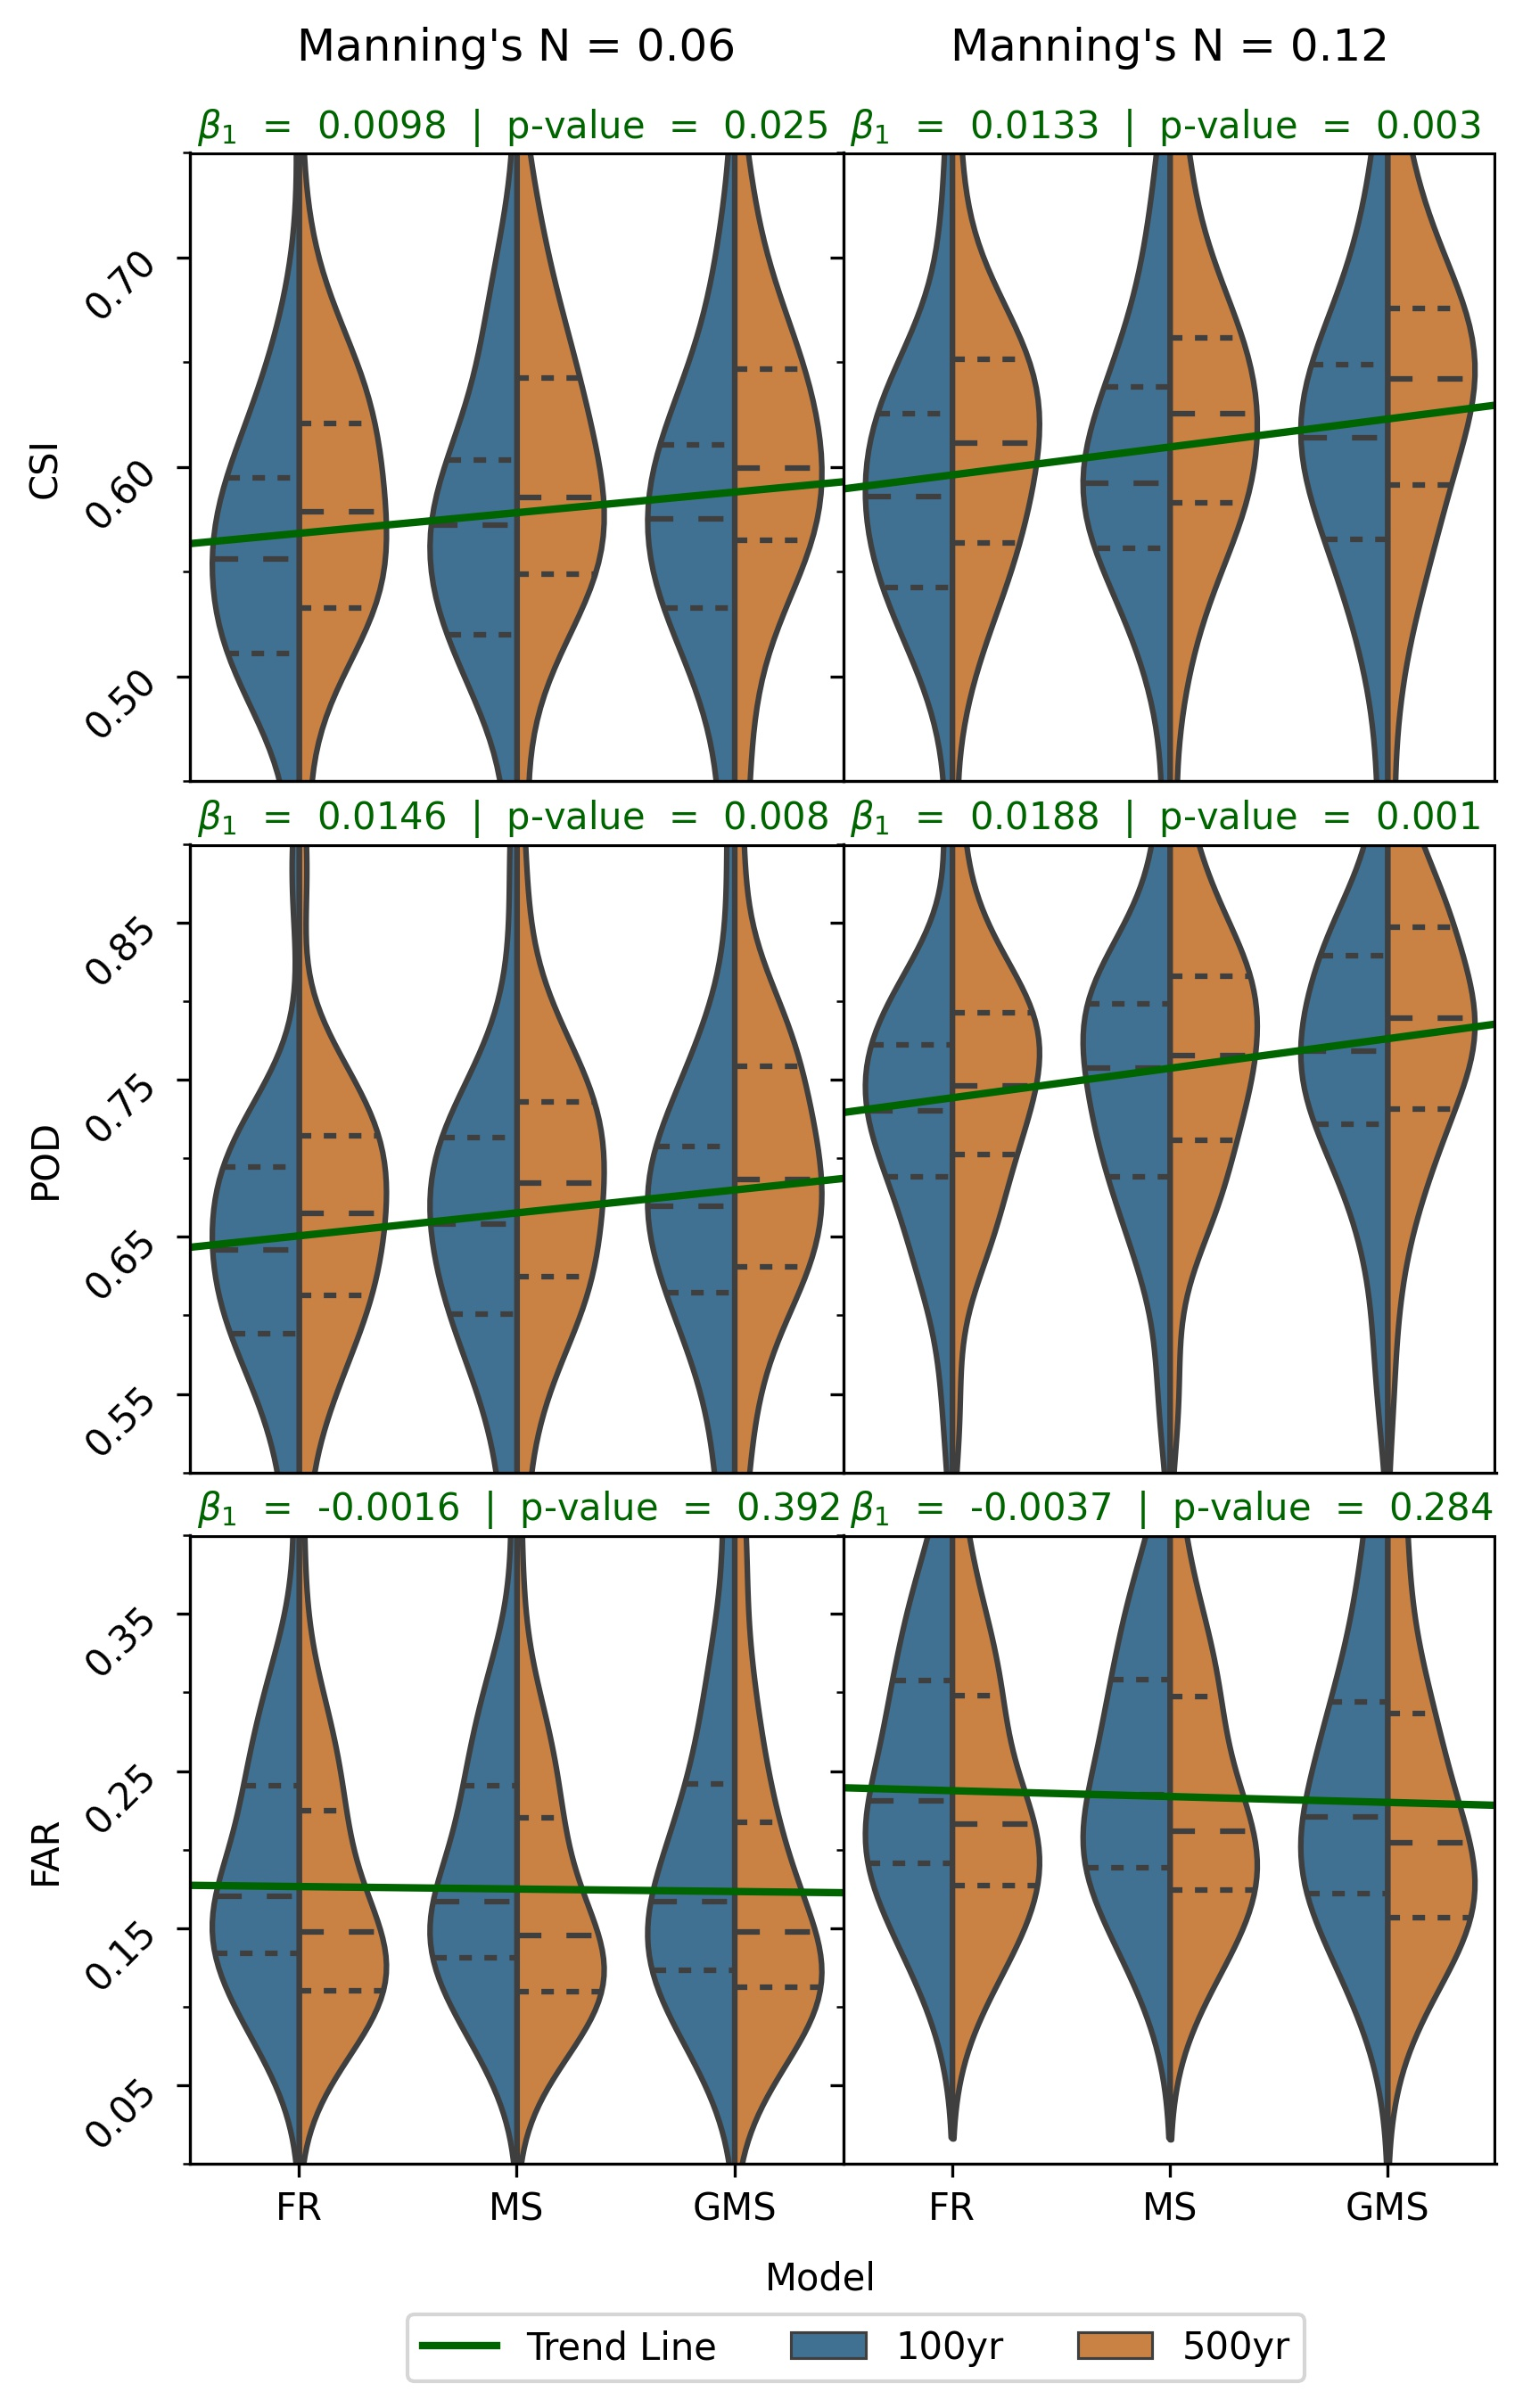
\includegraphics[scale=0.9]{figures/violin_plots.jpg}
\caption{Shows kernel density estimation of the distributions (sample size = 49) for 1\% (100 year) and 0.2\% (500 year) along with horizontal, dashed lines for the 25th, 50th, and 75th percentiles (in order from bottom to top).
The sub-figures separate the combination of three metrics (CSI, POD, and FAR) for two settings of Manning's n (0.06 and 0.12).
Trend lines for each metric - Mannings combination are shown (sample size = 294) along with associated slope and p-value of slope testing one-tailed significance.}
\label{fig:violin_plot}
\end{figure}
%
\begin{table}[h!]
\caption{Primary metrics, TPs, FPs, and FNs, aggregated for BLE domain to recompute CSI, POD, and FAR.}
\label{tab:aggregate_metrics}
\centering
%\begin{tabular}{|p{2cm}|p{2cm}|p{2cm}|p{2cm}|}
\begin{tabular}{|c|c||c|c|c|c|c|c|}
\hline
\multirow{2}{*}{Metric} & \multirow{2}{*}{Manning's n} & \multicolumn{2}{|c|}{FR} & \multicolumn{2}{|c|}{MS} & \multicolumn{2}{|c|}{GMS} \\
\cline{3-8}
  &  & 100yr & 500yr & 100yr & 500yr & 100yr & 500yr \\
\hline
\multirow{2}{*}{CSI} & 0.06 & 0.5576 & 0.5839 & 0.5717 & 0.5990 & 0.5796 & 0.6075 \\
\cline{2-8}
  & 0.12 & 0.5915 & 0.6149 & 0.6054 & 0.6288 & 0.6182 & 0.6435 \\
\hline
\multirow{2}{*}{POD} & 0.06 & 0.6354 & 0.6575 & 0.6524 & 0.6755 & 0.6633 & 0.6863 \\
\cline{2-8}
  & 0.12 & 0.7255 & 0.7446 & 0.7460 & 0.7648 & 0.7606 & 0.7810 \\
\hline
\multirow{2}{*}{FAR} & 0.06 & 0.1800 & 0.1609 & 0.1778 & 0.1589 & 0.1787 & 0.1589 \\
\cline{2-8}
  & 0.12 & 0.2379 & 0.2208 & 0.2374 & 0.2204 & 0.2324 & 0.2148 \\
\hline
\end{tabular}
\end{table}
%
% Interpretation of metrics
From Figure \ref{fig:violin_plot} and Table \ref{tab:aggregate_metrics}, we denote several meaningful trends. 
Using CSI as an overall proxy for skill of the FIM, we note that generally speaking the skill is correlated with a reduction of the stream orders of the processing units used for HAND.
In other words, the more you derive HAND on networks of unit drainage density and mosaic the resulting FIMs, the better those FIMs perform.
While this trend is evident for both sets of Manning's n values, the trend is slightly more significant for the higher value of 0.12.
Other trends related to this Figure include the general performance premium for 0.2\% events as opposed to lower 1\% events.
We also note how the higher Manning's n value enhances performance for both of these recurrence intervals across all models.

Dissecting the improvements and trends presented in the previous paragraph comes down mostly to improvement in POD or a reduction in absolute amount of FNs.
POD being the primary driver in skill enhancement is evident across models by comparing the slope of the POD lines with the slope of the FAR lines.
Even though aggregating metrics by HUC8 yields a statistically zero trend, one does see a slight reduction in FAR across models that reduce HAND's maximum stream order.
Additionally, we note that POD is a primary driver in enhancing performance across Manning's n values as well.
This significant improvement comes at a cost of false alarms as the FAR increases significantly across Manning's n values.
%
%%%%%%%%%%%%%%%%%%%%%%%%%%%%%%%%%%%%%%%%%%%%%%%%%%%%%%%%
\subsection{Computational Performance}
\label{ssec:compuational_performance}
%%%%%%%%%%%%%%%%%%%%%%%%%%%%%%%%%%%%%%%%%%%%%%%%%%%%%%%%
%
The NFIE experiments were able to produce HAND for 331 HUC6's in 1.34 CPU years \cite{liu2016cybergis} and estimates using work from \citeA{djokic2019arc} put producing HAND at the FR NWM at 0.55 CPU years. 
For our work, we were able to produce HAND at the full NWM resolution in 0.13 CPU years which represents a substantial speed-up compared to previous works.
For the MS resolution an additional, 0.05 CPU years is required on top of this bringing the total to about 0.18 CPU years to produce 2,188 HUC8s that span additional areas not covered in previous HAND versions including Hawaii and Puerto Rico.
GMS which generalizes HAND production to level path scale adds a significant amount of CPU time to the process bringing the estimate total to about 1.17 CPU years.
%

%
% Discussion
\clearpage % this clears figures before references
%%%%%%%%%%%%%%%%%%%%%%%%%%%%%%%%%%%%%%%%%%%%%%%%%%%%%%%%
%%%%%%%%%%%%%%%%%%%%%%%%%%%%%%%%%%%%%%%%%%%%%%%%%%%%%%%%
\section{Discussion}
\label{sec:discussion}
%%%%%%%%%%%%%%%%%%%%%%%%%%%%%%%%%%%%%%%%%%%%%%%%%%%%%%%%
%%%%%%%%%%%%%%%%%%%%%%%%%%%%%%%%%%%%%%%%%%%%%%%%%%%%%%%%
%
Overall, we note a positive relationship between FIM skill and a reduction of the stream order of the stream network we use to derive the HAND datasets.
Most of this change is accounted for by increasing POD thus reducing FNs especially along higher order rivers with higher flow magnitudes.
We note that reducing stream order does in turn suffer from diminishing returns in which the increase in mapping skill for applying stream order reduction to roughly 4-5\% of the stream network is about the same as the increase for applying stream order reduction to the remaining 95-96\% of the stream network.
This motivates further work in identifying what the optimal coverage of stream order reduction could be and how to parameterize that coverage. 
One option could be removing stream orders ones and possibly twos and threes from stream order reduction and simply using the inundation from FR from these areas.

In analyzing the data, we found a slight reduction in FAR was detected and more digging pointed to a bias in rating curves introduced by stream order reduction.
Figure \ref{fig:rating_curve_comparison} illustrates the general effect that stream order reduction has on synthetic rating curves.
Sub-figure \ref{fig:rating_curve_comparison}a shows how the average rating curves for all reaches for stage values 0 to 25 meters at one-third meter intervals tend to bias down (and to the right) with ever increasing stream order reduction (FR to MS to GMS). 
This bias is more pronounced for GMS since that implements stream order reduction down to the unit level for the entire FR network while MS only does so for 4-5\% of the network.
Attempting to diagnose this bias in the SRC leads one to Equation \ref{eq:reach_averaged_mannings_equation} which shows the reach averaged synthetic rating curve relationship between stage and discharge.
Across the three methods explored, FR, MS, and GMS, one identifies differences in the inputs and outputs and notes no difference in the stages and Manning's N values.
While the channel slope and reach lengths are not exactly the same across methods, their averaged differences are very negligible which only leaves room for deviations in volume and bed area.
Again, volume (V[y] or simply V) is synomous to reach-averaged cross-sectional area and bed area (B[y] or B) is analogous to reach-averaged hydraulic radius.
Discharge, Q, is directly related to volume and inversely related to bed area and each parameter is weighed according to the magnitude of its exponent which are $\frac{5}{3}$ and $\frac{2}{3}$ respectively. 
Figures \ref{fig:rating_curve_comparison} b and c show how volume and bed area compare across the three methods with GMS having significant higher values than MS which has higher values than FR.
Again the relative discrepency between FR vs MS and MS vs GMS is explained by the extent of their spatial coverages.
Both V and B values increase but since both are weighed differently by their respective exponents and pull Q in different directions.
We show in Figure \ref{fig:rating_curve_comparison}d the relationship of $\frac{V^{5/3}}{B^{2/3}}$ is plotted against stage, y, to show how these two parameters collectively pull the rating curve Q up and biases the rating curve down.
In other words, the magnitude and weight of the volume at each stage level exceeds the influence of the magnitude and weight of the bed area.
Both parameters are set to increase mainly due to much larger catchments leading to more pixels at each stage level as show in Figure \ref{fig:rating_curve_comparison}e.
Much of the increase in inundated pixels, volume, and bed area can be explained by much larger catchments than encompass neighboring tributaries.
These tributaries have a significant amount of bathymetry that is low-lying thus easily including the SRC derivation. 
They also contribute volume and bed area that is technically not perpendicular to the flux of streamflow being accounted for in the stream in question. 
Careful examination of Figure \ref{fig:gms_enhancement}b shows how much larger catchments include neighboring tributaries and the geometry associated with those tributaries. 
This geometry is not perpendicular to the flow that is associated with the main reach thus leading to biases in the SRC.
We consider this fact to have a nuanced effect on skill while reducing the rate of FPs it also can lead to FNs due to biases in the SRC.

Additional careful analysis of Figure \ref{fig:gms_enhancement}a, leads one to note many catchments that don't have inundation or significant inundation.
While the cause of these errors can be varied, we assert here that conflating 4 networks for use in evaluations leads to significant error.
As one may remember, Section \ref{sssec:cross_walking_networks} details how reach identifiers are conflated for the FIM network back to that of the NWM. 
One of the issues is when a reach of given stream order accidently conflates to that of a neighboring tributary that is of lower order which leads to areas of FNs.
The utilization of MS and GMS only conflates to NWM catchments directly associated with the level path in question which is inherently easy to do with those methods. 
Thus part of the improvement in MS and GMS methods is due to a slight improvement in cross-walking methodology.
The NWM stream network was derived using the NHD medium resolution dataset which was derived from coarser DEMs than those used here. 
Additional conflation is identified in cross-walking the stream network used by the BLE maps and those of HAND.
Until a singular stream network is used for the NWM, BLE benchmark, and for HAND based FIM, conflation will continue being a source of error.

For future development, we assert using experience from qualitative analysis that the synthetic rating curves offer a significant opportunity for improvement in HAND based FIM.
The bathymetry of the NED 10m DEM is known to be lacking proper representation thus leading to inadequate representation of volume and bed area with all three methods employed.
Manning's N which typically accounts for roughness could be tuned to account for these DEM limitations or could be held fixed to some local value associated with a given flood magnitude.
Some adjusting parameter must be introduced to enhance the estimation of the bathymetric representation.
Lidar DEMs from the USGS at 3m and 1m scale could be utilized to derive HAND as well which we conject should show better agreement with higher fidelity FIMs also derived from the same Lidar based DEMs.

Lastly, after errors introduced by conflation, poor roughness estimation, bathymetric/elevation adjustment are accounted for, HAND still has another fundamental limitation that is inherently baked into how it works.
For HAND to be derived and thus create a FIM for a given area, that area must entirely drain to the stream network and the stream network must also drain itself.
In other words, an entire area eligible for flooding must monotonically decrease in elevation. 
DEM's naturally don't do this and the dynamics of true flood events don't follow drainage patterns.
Enforcing this assumption for HAND leads to significant amount of DEM manipulations that introduce basic errors.
These errors are deep into the assumptions of HAND and thus more difficult to disentangle.
Ultimately, the use of more advanced 2-D hydrodynamic models should be considered for dealing with this limitation of HAND but would come at significant expense at the given high resolution across very large scales.
%
\begin{figure}[h!]
\centering
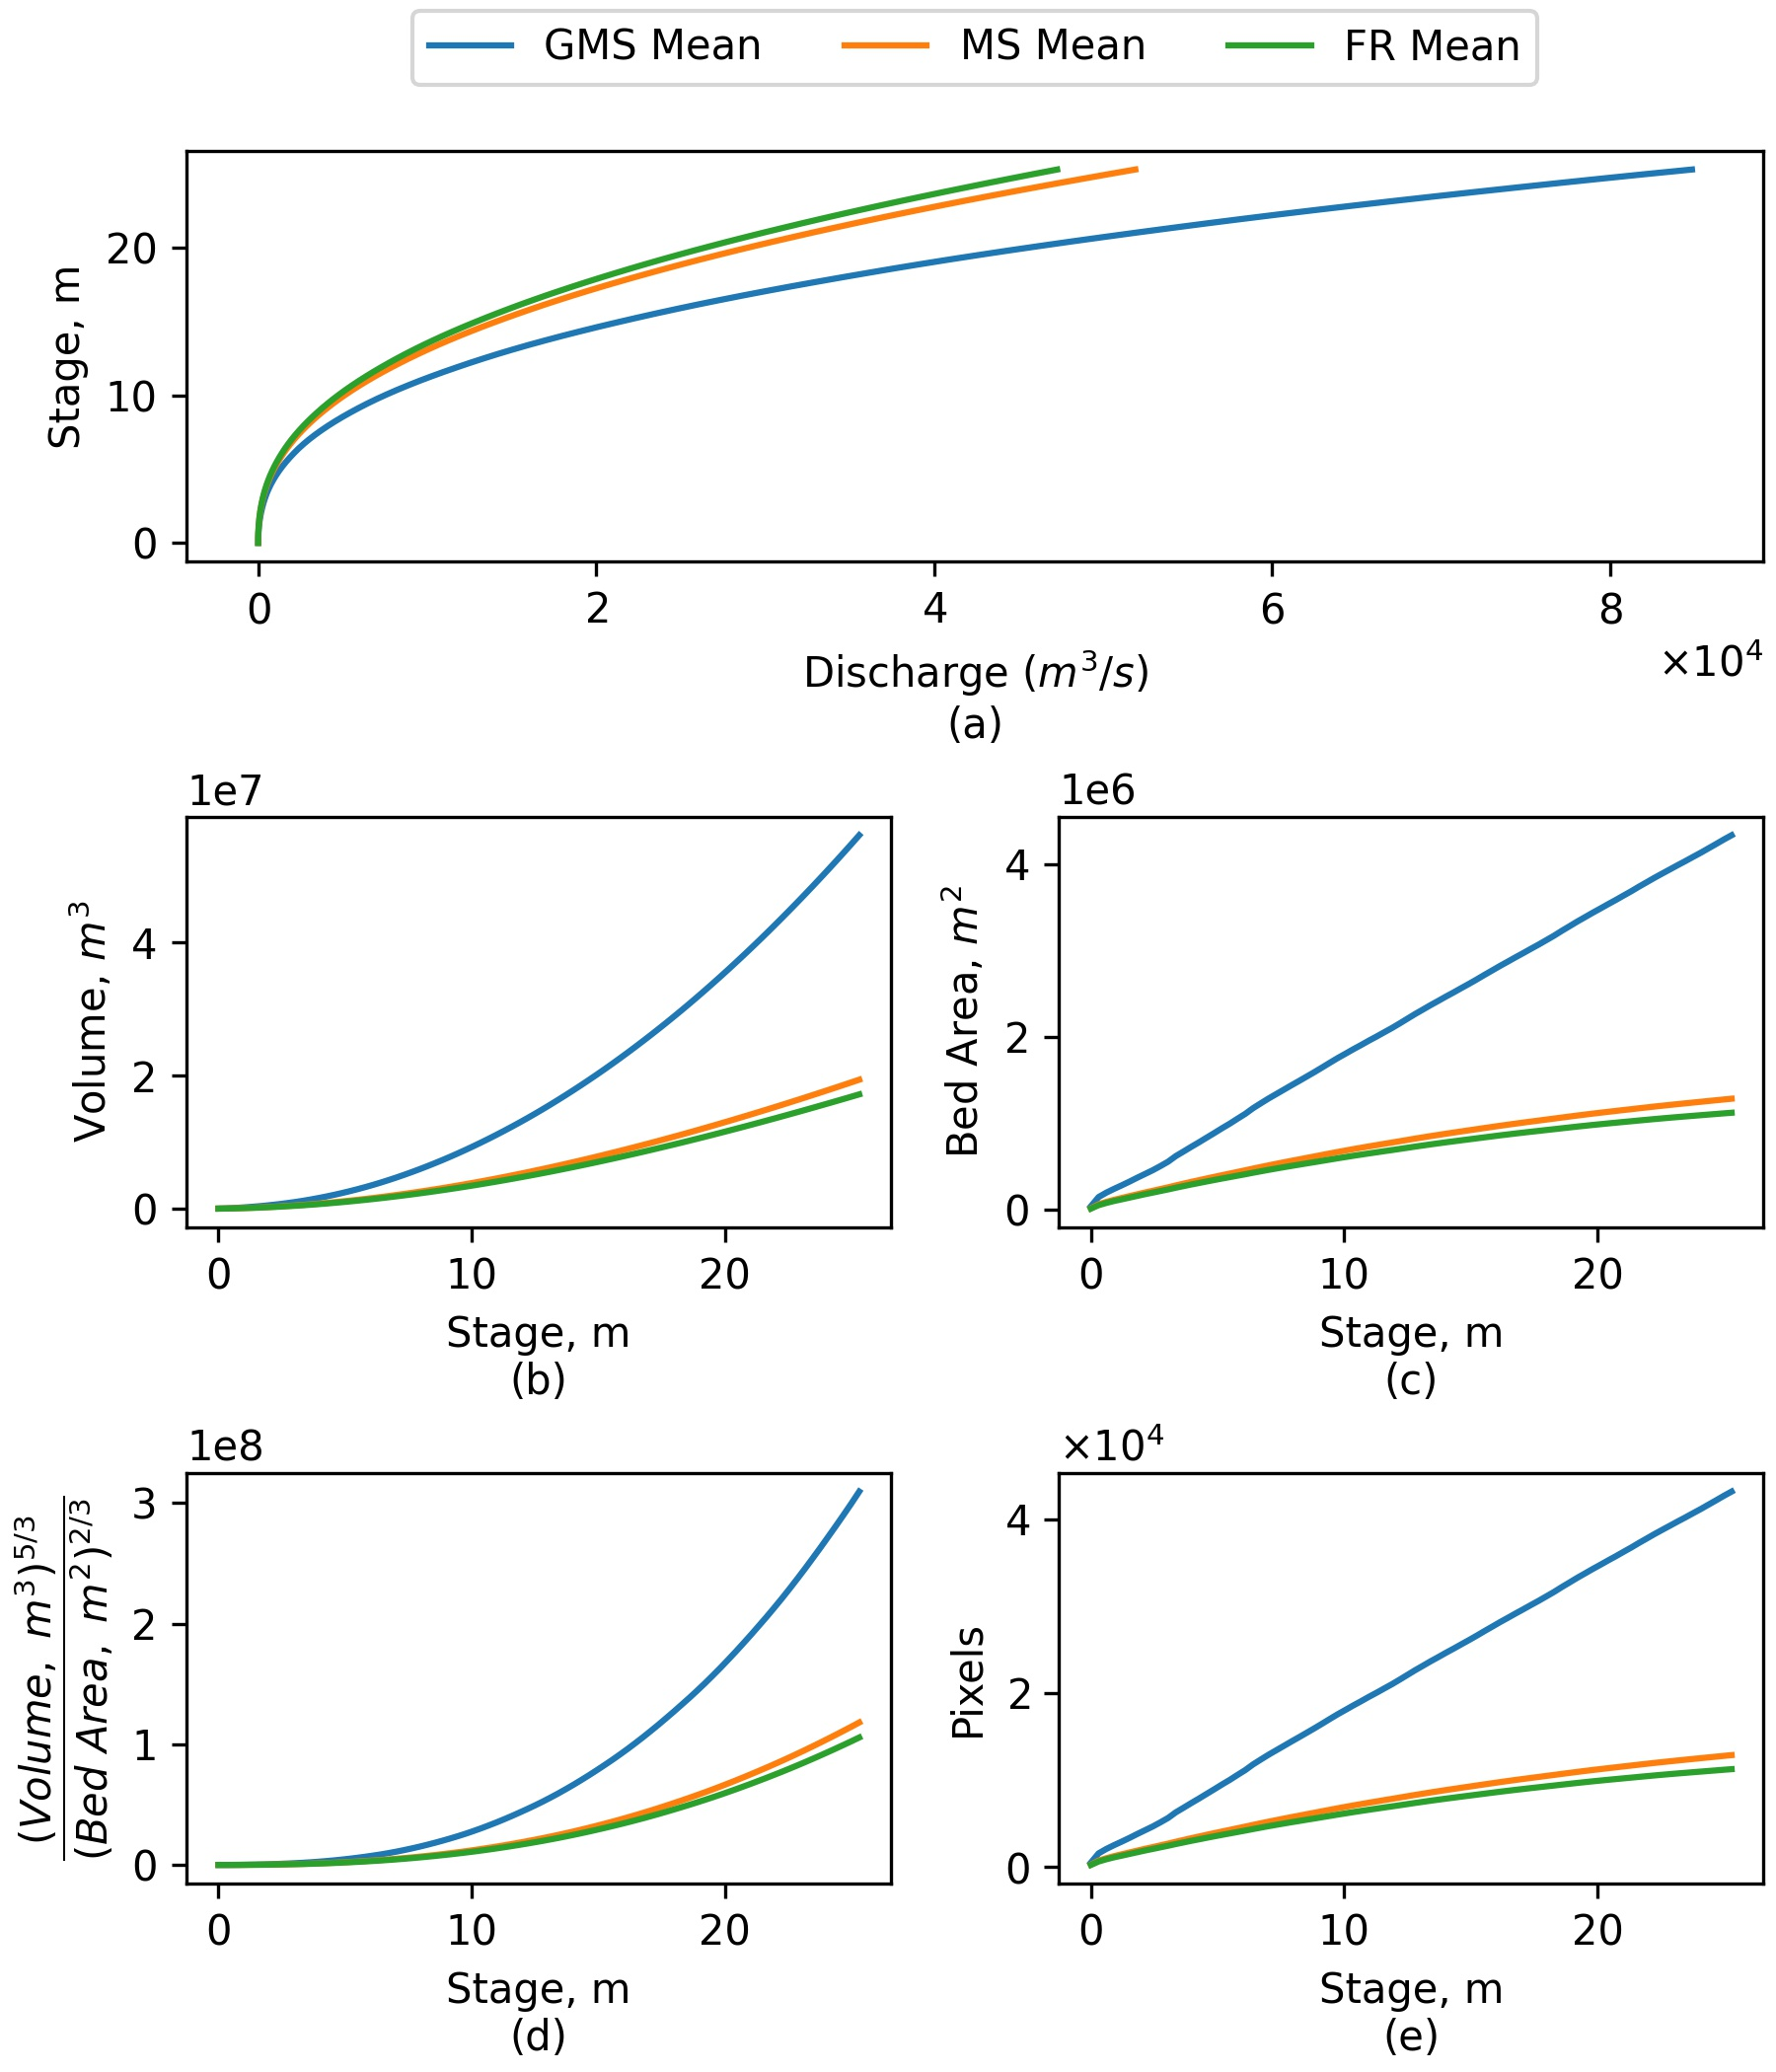
\includegraphics[scale=1.0]{figures/rating_curve_comparison.jpg}
\caption{Illustrates average quantities for the three methods, FR, MS, and GMS, for each stage value (m). 
The values are (a) Discharge $m^3s^{-1}$, (b) Volume $m^3$, (c) Bed Area $m^2$, (d) a function of Volume and Bed Area, and (e) number of pixels.
}
\label{fig:rating_curve_comparison}
\end{figure}
%
%
\begin{figure}[h!]
\centering
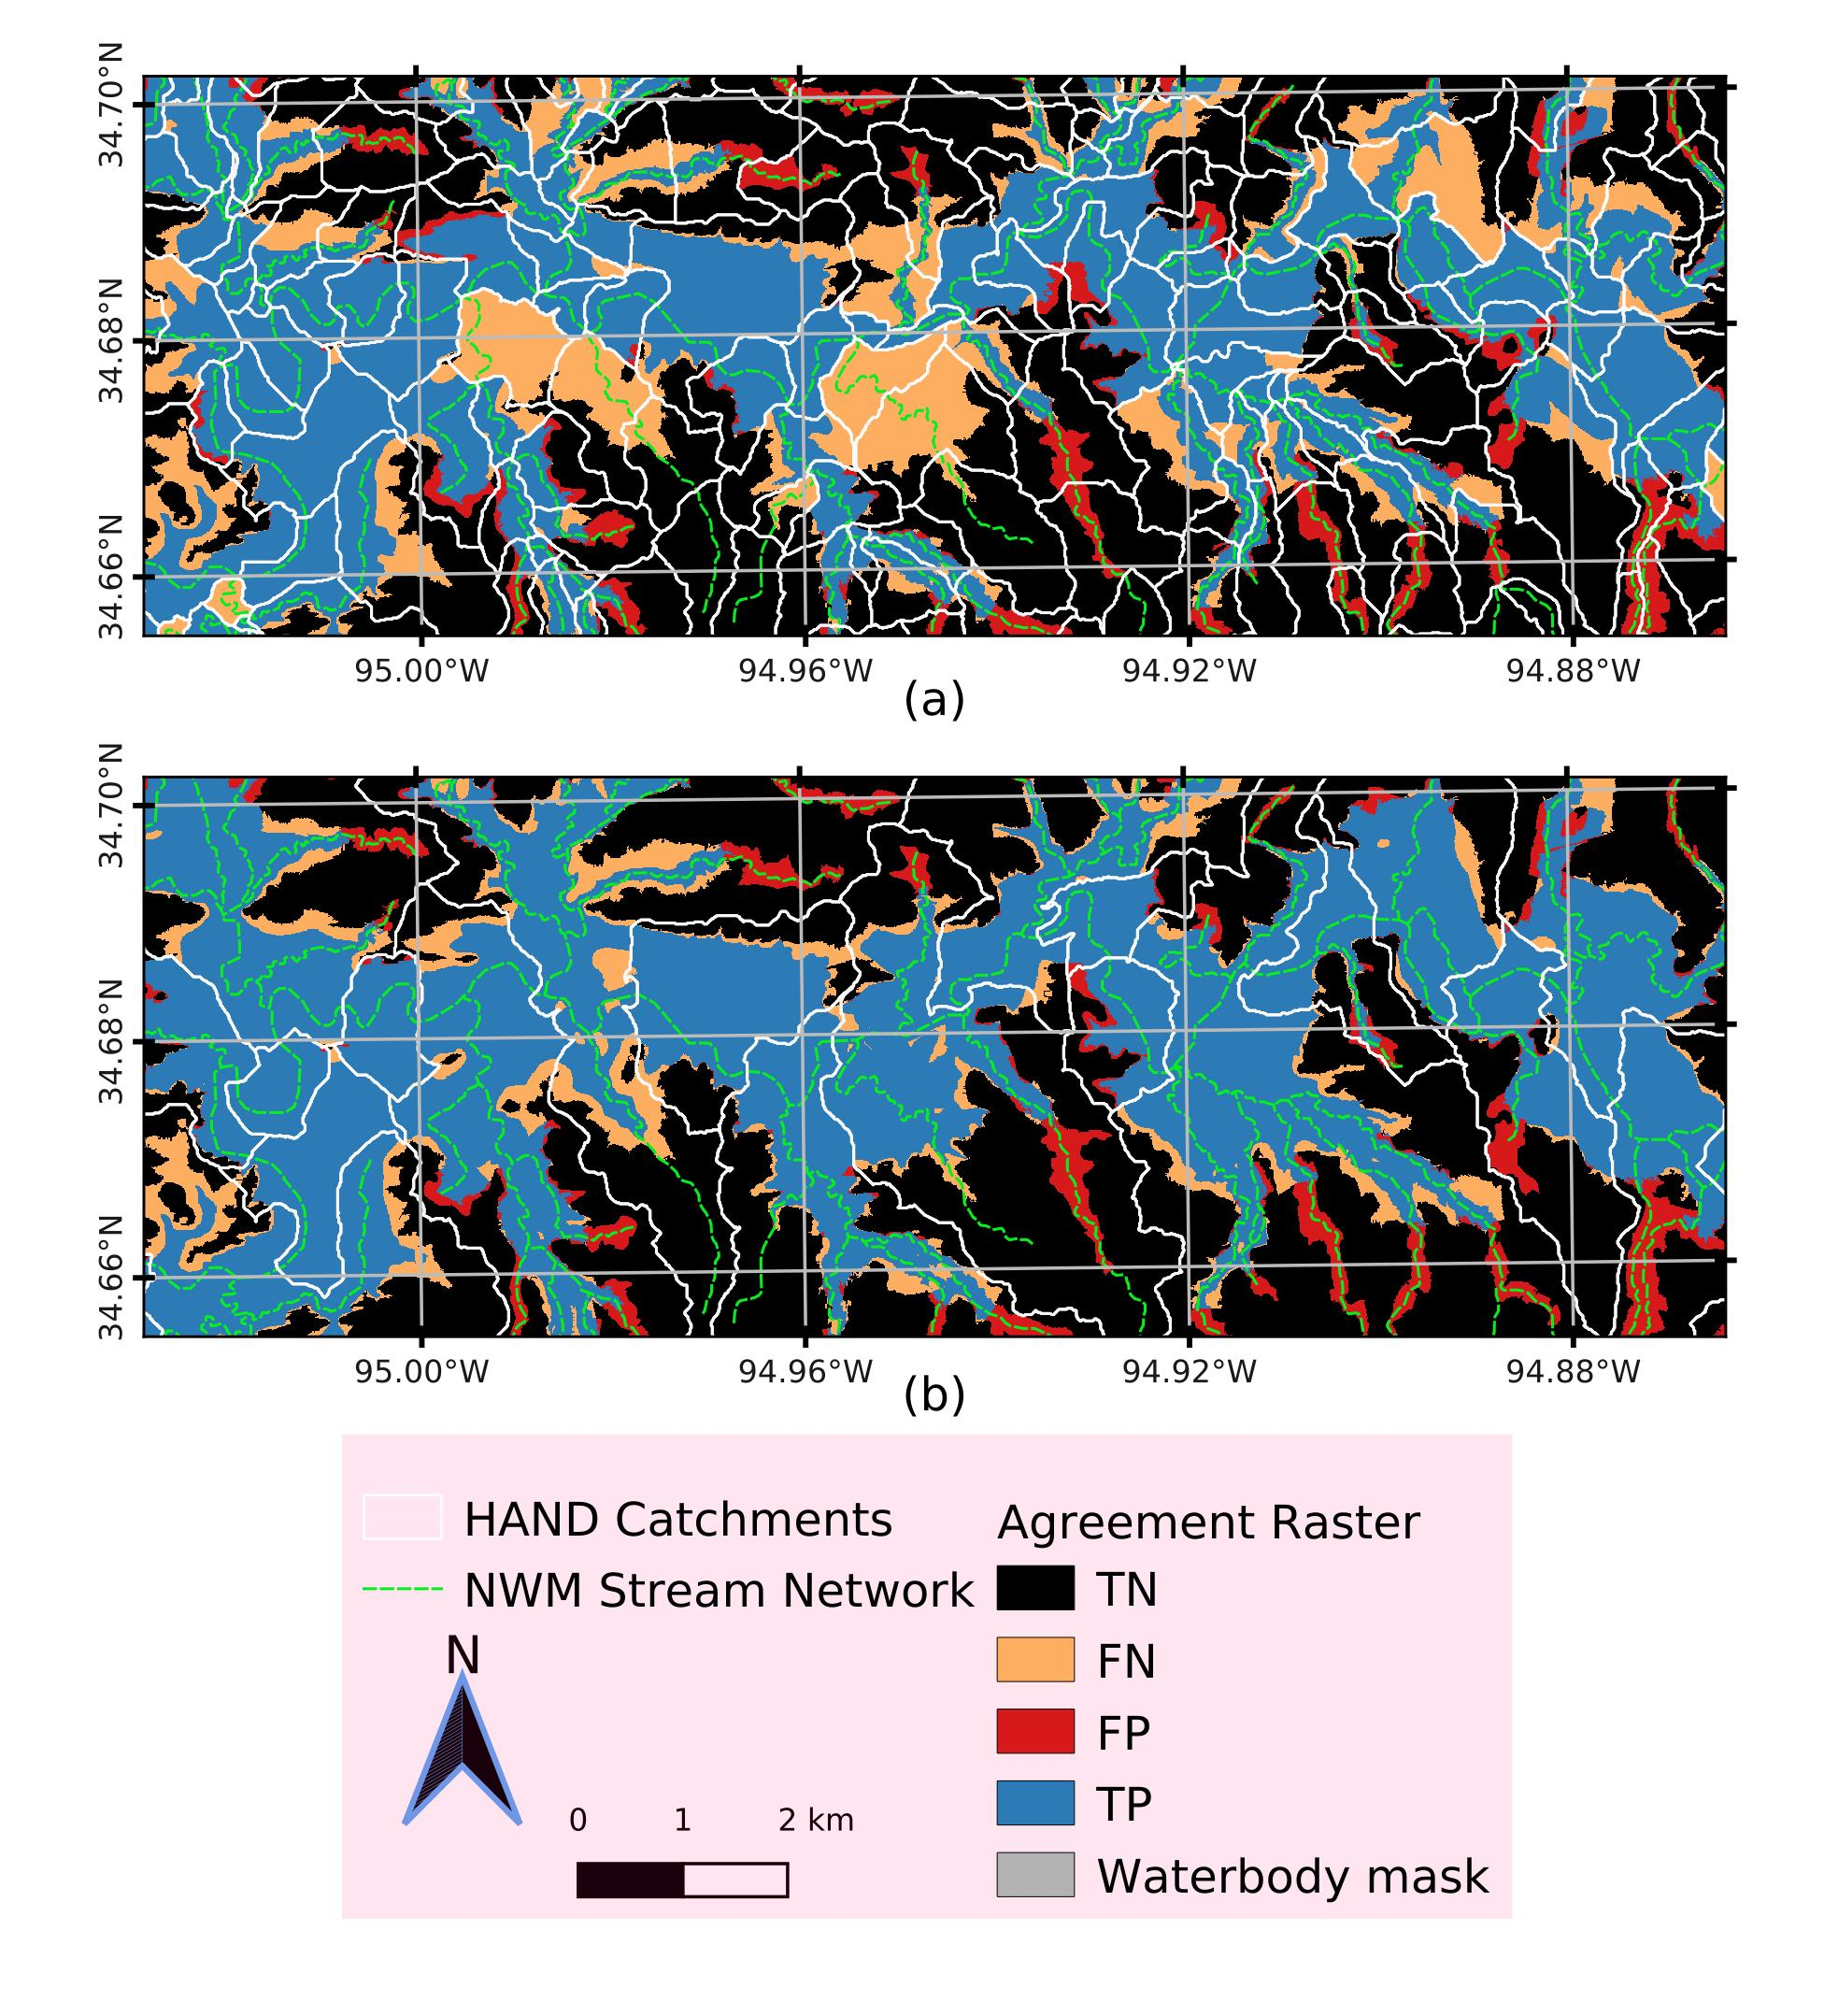
\includegraphics[scale=1.0]{figures/gms_enhancement.jpg}
\caption{OWP FIM `Cahaba' inundation agreement, TP, FP, FN, and TN, with BLE HEC-RAS maps in HUC 11140105.
Catchment boundaries and stream lines are shown in white and dotted green, respectively.
Sub-figure (a) shows agreement of FR HAND denoting significant areas of under-prediction due to junctions and catchment boundaries.
Meanwhile, (b) shows the agreement for GMS and much larger catchments leading to much better inundation agreement for this given reach. 
Overall, this illustrates the benefits of stream order reduction for deriving HAND datasets.
}
\label{fig:gms_enhancement}
\end{figure}
%

%
% Conclusions
\clearpage % this clears figures before references
\section{Conclusions}

%
%%

%  Numbered lines in equations:
%  To add line numbers to lines in equations,
%  \begin{linenomath*}
%  \begin{equation}
%  \end{equation}
%  \end{linenomath*}


%% Enter Figures and Tables near as possible to where they are first mentioned:
%
% DO NOT USE \psfrag or \subfigure commands.
%
% Figure captions go below the figure.
%\section{= enter section title =}
%Text here ===>>>
%\section{= enter section title =}
%Text here ===>>>
%%

%  Numbered lines in equations:
%  To add line numbers to lines in equations,
%  \begin{linenomath*}
%  \begin{equation}
%  \end{equation}
%  \end{linenomath*}



%% Enter Figures and Tables near as possible to where they are first mentioned:
%
% DO NOT USE \psfrag or \subfigure commands.
%
% Figure captions go below the figure.
% Table titles go above tables;  other caption information
%  should be placed in last line of the table, using
% \multicolumn2l{$^a$ This is a table note.}
%
%----------------
% EXAMPLE FIGURES
%
% \begin{figure}
% \includegraphics{example.png}
% \caption{caption}
% \end{figure}
%
% Giving latex a width will help it to scale the figure properly. A simple trick is to use \textwidth. Try this if large figures run off the side of the page.
% \begin{figure}
% \noindent\includegraphics[width=\textwidth]{anothersample.png}
%\caption{caption}
%\label{pngfiguresample}
%\end{figure}
%
%
% If you get an error about an unknown bounding box, try specifying the width and height of the figure with the natwidth and natheight options. This is common when trying to add a PDF figure without pdflatex.
% \begin{figure}
% \noindent\includegraphics[natwidth=800px,natheight=600px]{samplefigure.pdf}
%\caption{caption}
%\label{pdffiguresample}
%\end{figure}
%
%
% PDFLatex does not seem to be able to process EPS figures. You may want to try the epstopdf package.
%

%
% ---------------
% EXAMPLE TABLE
%
% \begin{table}
% \caption{Time of the Transition Between Phase 1 and Phase 2$^{a}$}
% \centering
% \begin{tabular}{l c}
% \hline
%  Run  & Time (min)  \\
% \hline
%   $l1$  & 260   \\
%   $l2$  & 300   \\
%   $l3$  & 340   \\
%   $h1$  & 270   \\
%   $h2$  & 250   \\
%   $h3$  & 380   \\
%   $r1$  & 370   \\
%   $r2$  & 390   \\
% \hline
% \multicolumn{2}{l}{$^{a}$Footnote text here.}
% \end{tabular}
% \end{table}

%% SIDEWAYS FIGURE and TABLE
% AGU prefers the use of {sidewaystable} over {landscapetable} as it causes fewer problems.
%
% \begin{sidewaysfigure}
% \includegraphics[width=20pc]{figsamp}
% \caption{caption here}
% \label{newfig}
% \end{sidewaysfigure}
%
%  \begin{sidewaystable}
%  \caption{Caption here}
% \label{tab:signif_gap_clos}
%  \begin{tabular}{ccc}
% one&two&three\\
% four&five&six
%  \end{tabular}
%  \end{sidewaystable}

%% If using numbered lines, please surround equations with \begin{linenomath*}...\end{linenomath*}
%\begin{linenomath*}
%\begin{equation}
%y|{f} \sim g(m, \sigma),
%\end{equation}
%\end{linenomath*}

%%% End of body of article

%%%%%%%%%%%%%%%%%%%%%%%%%%%%%%%%
%% Optional Appendix goes here
%
% The \appendix command resets counters and redefines section heads
%
% After typing \appendix
%
%\section{Here Is Appendix Title}
% will show
% A: Here Is Appendix Title
%
%\appendix
%\section{Here is a sample appendix}

%%%%%%%%%%%%%%%%%%%%%%%%%%%%%%%%%%%%%%%%%%%%%%%%%%%%%%%%%%%%%%%%
%
% Optional Glossary, Notation or Acronym section goes here:
%
%%%%%%%%%%%%%%
% Glossary is only allowed in Reviews of Geophysics
%  \begin{glossary}
%  \term{Term}
%   Term Definition here
%  \term{Term}
%   Term Definition here
%  \term{Term}
%   Term Definition here
%  \end{glossary}

%
%%%%%%%%%%%%%%
% Acronyms
%   \begin{acronyms}
%   \acro{Acronym}
%   Definition here
%   \acro{EMOS}
%   Ensemble model output statistics
%   \acro{ECMWF}
%   Centre for Medium-Range Weather Forecasts
%   \end{acronyms}

%
%%%%%%%%%%%%%%
% Notation
%   \begin{notation}
%   \notation{$a+b$} Notation Definition here
%   \notation{$e=mc^2$}
%   Equation in German-born physicist Albert Einstein's theory of special
%  relativity that showed that the increased relativistic mass ($m$) of a
%  body comes from the energy of motion of the body—that is, its kinetic
%  energy ($E$)—divided by the speed of light squared ($c^2$).
%   \end{notation}




%%%%%%%%%%%%%%%%%%%%%%%%%%%%%%%%%%%%%%%%%%%%%%%%%%%%%%%%%%%%%%%%
%
%  ACKNOWLEDGMENTS
%
% The acknowledgments must list:
%
% >>>>	A statement that indicates to the reader where the data
% 	supporting the conclusions can be obtained (for example, in the
% 	references, tables, supporting information, and other databases).
%
% 	All funding sources related to this work from all authors
%
% 	Any real or perceived financial conflicts of interests for any
%	author
%
% 	Other affiliations for any author that may be perceived as
% 	having a conflict of interest with respect to the results of this
% 	paper.
%
%
% It is also the appropriate place to thank colleagues and other contributors.
% AGU does not normally allow dedications.


\acknowledgments
This work was funded by the OWP which is part of NOAA's National Weather Service.
Lynker was the beneficiary of this funding and we'd like to thank them for facilitating computational resources used in the development of this work.
We would like to thank some notable facilitators to this work including Chief Scientist at OWP, Dr. Fred Ogden for his technical expertise.
Additionally, David Blodgett from the USGS Water Mission Area was instrumental in helping define level paths and other hydrographic work.
More information on code availability, usage, and data retrieval for OWP FIM `Cahaba' is available at https://github.com/NOAA-OWP/cahaba.
The Earth and Space Science Informatics Partnership (ESIP) helps store our data for public use and dissemination so a thank you is warrented to ESIP for helping provide transparent datasets for further collaboration with the research community.


%% ------------------------------------------------------------------------ %%
%% References and Citations

%%%%%%%%%%%%%%%%%%%%%%%%%%%%%%%%%%%%%%%%%%%%%%%
%
% \bibliography{<name of your .bib file>} don't specify the file extension
%
% don't specify bibliography style
%%%%%%%%%%%%%%%%%%%%%%%%%%%%%%%%%%%%%%%%%%%%%%%
%
\clearpage % this clears figures before references
\bibliography{bibliography/owp_fim4_2021}
%
%Reference citation instructions and examples:
%
% Please use ONLY \cite and \citeA for reference citations.
% \cite for parenthetical references
% ...as shown in recent studies (Simpson et al., 2019)
% \citeA for in-text citations
% ...Simpson et al. (2019) have shown...
%
%
%...as shown by \citeA{jskilby}.
%...as shown by \citeA{lewin76}, \citeA{carson86}, \citeA{bartoldy02}, and \citeA{rinaldi03}.
%...has been shown \cite{jskilbye}.
%...has been shown \cite{lewin76,carson86,bartoldy02,rinaldi03}.
%... \cite <i.e.>[]{lewin76,carson86,bartoldy02,rinaldi03}.
%...has been shown by \cite <e.g.,>[and others]{lewin76}.
%
% apacite uses < > for prenotes and [ ] for postnotes
% DO NOT use other cite commands (e.g., \citet, \citep, \citeyear, \nocite, \citealp, etc.).
%



\end{document}



%%%% More Information and Advice:

%% ------------------------------------------------------------------------ %%
%
%  SECTION HEADS
%
%% ------------------------------------------------------------------------ %%

% Capitalize the first letter of each word (except for
% prepositions, conjunctions, and articles that are
% three or fewer letters).

% AGU follows standard outline style; therefore, there cannot be a section 1 without
% a section 2, or a section 2.3.1 without a section 2.3.2.
% Please make sure your section numbers are balanced.
% ---------------
% Level 1 head
%
% Use the \section{} command to identify level 1 heads;
% type the appropriate head wording between the curly
% brackets, as shown below.
%
%An example:
%\section{Level 1 Head: Introduction}
%
% ---------------
% Level 2 head
%
% Use the \subsection{} command to identify level 2 heads.
%An example:
%\subsection{Level 2 Head}
%
% ---------------
% Level 3 head
%
% Use the \subsubsection{} command to identify level 3 heads
%An example:
%\subsubsection{Level 3 Head}
%
%---------------
% Level 4 head
%
% Use the \subsubsubsection{} command to identify level 3 heads
% An example:
%\subsubsubsection{Level 4 Head} An example.
%
%% ------------------------------------------------------------------------ %%
%
%  IN-TEXT LISTS
%
%% ------------------------------------------------------------------------ %%
%
% Do not use bulleted lists; enumerated lists are okay.
% \begin{enumerate}
% \item
% \item
% \item
% \end{enumerate}
%
%% ------------------------------------------------------------------------ %%
%
%  EQUATIONS
%
%% ------------------------------------------------------------------------ %%

% Single-line equations are centered.
% Equation arrays will appear left-aligned.

Math coded inside display math mode \[ ...\]
 will not be numbered, e.g.,:
 \[ x^2=y^2 + z^2\]

 Math coded inside \begin{equation} and \end{equation} will
 be automatically numbered, e.g.,:
 \begin{equation}
 x^2=y^2 + z^2
 \end{equation}


% To create multiline equations, use the
% \begin{eqnarray} and \end{eqnarray} environment
% as demonstrated below.
\begin{eqnarray}
  x_{1} & = & (x - x_{0}) \cos \Theta \nonumber \\
        && + (y - y_{0}) \sin \Theta  \nonumber \\
  y_{1} & = & -(x - x_{0}) \sin \Theta \nonumber \\
        && + (y - y_{0}) \cos \Theta.
\end{eqnarray}

%If you don't want an equation number, use the star form:
%\begin{eqnarray*}...\end{eqnarray*}

% Break each line at a sign of operation
% (+, -, etc.) if possible, with the sign of operation
% on the new line.

% Indent second and subsequent lines to align with
% the first character following the equal sign on the
% first line.

% Use an \hspace{} command to insert horizontal space
% into your equation if necessary. Place an appropriate
% unit of measure between the curly braces, e.g.
% \hspace{1in}; you may have to experiment to achieve
% the correct amount of space.


%% ------------------------------------------------------------------------ %%
%
%  EQUATION NUMBERING: COUNTER
%
%% ------------------------------------------------------------------------ %%

% You may change equation numbering by resetting
% the equation counter or by explicitly numbering
% an equation.

% To explicitly number an equation, type \eqnum{}
% (with the desired number between the brackets)
% after the \begin{equation} or \begin{eqnarray}
% command.  The \eqnum{} command will affect only
% the equation it appears with; LaTeX will number
% any equations appearing later in the manuscript
% according to the equation counter.
%

% If you have a multiline equation that needs only
% one equation number, use a \nonumber command in
% front of the double backslashes (\\) as shown in
% the multiline equation above.

% If you are using line numbers, remember to surround
% equations with \begin{linenomath*}...\end{linenomath*}

%  To add line numbers to lines in equations:
%  \begin{linenomath*}
%  \begin{equation}
%  \end{equation}
%  \end{linenomath*}



